%% Elsevier cas-sc single-column manuscript
%% Sections 1-3 (Introduction / Theoretical background / Proposed method)
%% drafted for the CMGAN-T60 (Fourier-KAN) paper.

\documentclass[a4paper,fleqn]{cas-sc}

\usepackage[numbers]{natbib}
\usepackage{amsmath}
\usepackage{amssymb}
\usepackage{graphicx}
\usepackage{float}
\usepackage{booktabs}
\usepackage{multirow}
\usepackage{url}
\usepackage{lineno}

\linenumbers

%% Float placement — force LaTeX to place figures as early as possible
\renewcommand{\topfraction}{0.95}
\renewcommand{\bottomfraction}{0.95}
\renewcommand{\textfraction}{0.02}
\renewcommand{\floatpagefraction}{0.75}

%% Author definitions
\def\tsc#1{\csdef{#1}{\textsc{\lowercase{#1}}\xspace}}

\begin{document}
\let\WriteBookmarks\relax

\shorttitle{Conformer-based blind $T_{60}$ estimation with Fourier-KAN}
\shortauthors{X. Xie, X. Lu and J. Sang}

\title[mode=title]{Multi-task blind reverberation time estimation with a denoising auxiliary task and a Fourier Kolmogorov--Arnold regression head}

%% ------------- Authors -------------
\author[1]{Xinni Xie}[%
  type=editor]

\author[1]{Xikun Lu}

\author[1]{Jinqiu Sang}
\cormark[1]
\ead{jqsang@mail.ecnu.edu.cn}

\affiliation[1]{organization={East China Normal University},
                city={Shanghai},
                country={China}}

\cortext[cor1]{Corresponding author}

\begin{abstract}
Reverberation time $T_{60}$ is one of the most informative room-acoustic
parameters, yet blind estimation from a single-channel noisy reverberant
recording remains difficult because the late reverberation tail is
intrinsically energy-weak and is easily masked by additive noise. We
propose a multi-task learning framework for blind $T_{60}$ estimation in
which $T_{60}$ regression is the main task and denoising reconstruction
(noisy reverberant speech $\to$ clean reverberant speech) is an auxiliary
task, both sharing a dual-path time--frequency Conformer backbone. The
complex short-time Fourier spectrum of the noisy reverberant utterance is
processed by a dense convolutional encoder and two time--frequency
Conformer blocks (TSCBs); the bottleneck features are aggregated by a
multi-statistic pooling layer and mapped to $T_{60}$ by a two-layer
Fourier-KAN head, while the same bottleneck feeds a mask decoder and a
complex decoder that reconstruct the enhanced speech. The dense,
per-time-frequency-bin supervision of the denoising auxiliary task forces
the shared layers to learn fine-grained time--frequency discriminative
features, and we show that this denoising-driven representation in turn
substantially improves $T_{60}$ estimation. Compared with a multi-layer
perceptron (MLP) head of similar capacity, the Fourier basis expresses
each edge activation as a learnable trigonometric series, which is well
matched to the smooth but non-linear dependence between pooled acoustic
statistics and the target $T_{60}$. On four noisy reverberant test sets
covering both simulated and measured room impulse responses with seen and
unseen noise types, the proposed model attains an average root-mean-squared
error (RMSE) of $92.91$\,ms, a mean absolute error (MAE) of
$56.68$\,ms and a Pearson correlation of $0.9625$; relative
to a single-task ablation baseline ($861\,793$ parameters, RMSE
$111.15$\,ms) this is a $16.4$\,\% RMSE reduction. The encoder and
Conformer blocks are shared between the two tasks, and the denoising
auxiliary task adds two decoders of about $0.54$\,M parameters, giving
$1.41$\,M parameters in total. Gradient-probe analysis shows that the
two task gradients remain nearly orthogonal throughout training (no
systematic conflict), so the two tasks can be optimised jointly without
interference; a task-weight ablation further shows that $T_{60}$
accuracy improves as the denoising task is given a larger
weight, and representation analysis indicates that this gain comes from
the denoising task reshaping the shared features rather than from any
gradient-dominance effect.
\end{abstract}

\begin{keywords}
Blind reverberation time estimation \sep Multi-task learning \sep
Denoising auxiliary supervision \sep Conformer \sep Kolmogorov--Arnold
network \sep Fourier basis \sep Noise robustness
\end{keywords}

\maketitle

% =====================================================================
\section{Introduction}
% =====================================================================

When a sound is emitted in an enclosure, the receiver captures not only
the direct path but also a dense set of reflections from the surrounding
boundaries~\citep{kuttruff2013room}. These reflections decay over time and
together form the room reverberation. The time required for the sound
energy to decay by 60\,dB after the source has been switched off is
defined as the reverberation time $T_{60}$~\citep{iso3382_2_2008}. As a
single scalar that summarises the energy-decay behaviour of a room,
$T_{60}$ is one of the most widely used parameters to characterise the
acoustic property of an enclosure and has a direct impact on speech
quality, intelligibility, and the performance of downstream audio
applications such as dereverberation, speech recognition, sound source
localisation, and virtual or augmented reality
rendering~\citep{benzeghiba2007asrreview, anthes2016vr}. The standardised
ways of measuring $T_{60}$ are the interrupted-noise method and the
integrated impulse response method~\citep{schroeder1965rt}, both of which
require omnidirectional sources, calibrated microphones and trained
operators. Such on-site measurements are nevertheless not portable, and are
costly and complex to implement whenever large-scale or in-situ
measurement is needed. \emph{Blind} estimation methods have therefore
emerged, in which
$T_{60}$ is inferred directly from a recorded speech signal without any
dedicated excitation or knowledge of the room
geometry~\citep{eaton2016ace}.

Over the past two decades, a large body of work on blind $T_{60}$
estimation has accumulated. The traditional family relies on statistical
signal processing: model-based estimators describe the late part of the
room impulse response (RIR) as a damped Gaussian
process~\citep{polack1988these} and recover $T_{60}$ from the decay rate
of the energy envelope, while feature-mapping based estimators derive
$T_{60}$ from a hand-designed acoustic descriptor such as the negative-side
variance of the decay rate, the pitch strength of harmonic
components or the spectral decay
distribution~\citep{ratnam2003blind, wen2008negativeside, eaton2013sdd,
falk2010temporal, lollmann2010iwaenc}. These methods have been thoroughly
benchmarked by the ACE challenge~\citep{eaton2016ace}, which also revealed
two recurring difficulties: (i) most estimators are positively biased by
additive noise because the noise-like reverberation tail is buried in the
noise, and (ii) the analytic decay model is fragile in non-stationary or
low-SNR scenarios. Even noise-robust extensions such as the
spectral-decay-distribution estimator with reduced computational
cost~\citep{eaton2013sdd} or the subband-decomposition based
estimator~\citep{prego2015subband} still require a relatively accurate
prior estimate of the noise level, which is itself a hard problem when
the noise is non-stationary. The masking of the reverberation tail by
additive noise is thus a central obstacle for blind $T_{60}$ estimation,
and robustly recovering the decay structure under noisy conditions has
become a recurring problem for subsequent methods.

Deep learning (DL) has subsequently emerged as a data-driven alternative.
\citet{gamper2018cnn} fed log-mel features to a six-layer convolutional
neural network and won the ACE single-channel track; \citet{xiong2018ercnn}
posed the joint $T_{60}$ and direct-to-reverberant ratio estimation as a
classification problem on time--frequency features; \citet{deng2020crnn}
introduced a convolutional recurrent network for online estimation on
variable-length utterances; \citet{srivastava2021blindroom} extended the
formulation to multi-channel inputs; \citet{goetz2023online} tackled
parameter estimation under dynamic acoustic conditions with three
convolutional recurrent variants; \citet{saini2023mobileaudiotransformer}
have demonstrated that a MobileViT-style transformer can run on a
smartphone in real time, while \citet{duangpummet2022stochastic} have
moved from full-band $T_{60}$ towards a joint estimation of $T_{60}$,
early-decay time, clarity and speech transmission index. Although these
models differ considerably in network architecture, most of them adopt
the same regressor design, namely a stack of fully connected layers on
top of the time--frequency backbone that maps the aggregated features to
a scalar $T_{60}$. To improve robustness under noisy conditions, one line
of work further exploits denoising to assist $T_{60}$ estimation:
\citet{zheng2022noiseaware} used a two-stage framework that first
separates the clean reverberant speech and then estimates $T_{60}$ from
it, but the two stages are trained separately, so the denoising gradients
cannot directly optimise the features on which $T_{60}$ relies;
\citet{zhang2024damtl} instead treated denoising as an auxiliary task that
shares a backbone with $T_{60}$ regression and is trained end to end, and
observed that denoising improves $T_{60}$ estimation, but their backbone
is relatively simple and they did not analyse how the two tasks interact
in the shared layers, so the mechanism behind the denoising-induced gain
remains unclear.

Although the data-driven models above clearly outperform the statistical
signal processing baselines in clean or high-SNR conditions, two general
challenges persist across this body of work. First, the late
reverberation tail is intrinsically energy-weak and is easily masked by
real-world noise, so estimation accuracy still degrades noticeably in
low-SNR or unseen-noise scenarios; existing estimators mainly rely on the
backbone's own capacity to obtain noise robustness implicitly, without
any explicit modelling or separation of the noise, and it is therefore
unclear whether this alone drives the lower layers to learn the
fine-grained time--frequency discriminative features on which an accurate
$T_{60}$, itself dependent on the detailed shape of the decay envelope,
ultimately relies. Second, as noted above, almost all existing estimators
place a stack of fully connected layers on top of the time--frequency
backbone as the regressor, which applies a single fixed non-linearity per
neuron and offers limited expressive power for the smooth but non-trivial
mapping from pooled bottleneck statistics to a scalar $T_{60}$.

To address these challenges, we propose a multi-task learning framework
for blind $T_{60}$ estimation that pairs $T_{60}$ regression with a
denoising reconstruction auxiliary task over a shared time--frequency
Conformer backbone. For the first challenge, the denoising auxiliary task
provides dense per-time-frequency-bin supervision that forces the shared
layers to learn to separate noise from the reverberant spectrum, thereby
exposing the masked decay structure; since sharing parameters across
tasks can cause negative transfer~\citep{ruder2017overview, yu2020pcgrad},
we further conduct gradient-probe and representation analyses to verify
the underlying mechanism. For the second challenge, we replace the
conventional fully connected regression head with a Fourier-KAN head,
whose learnable trigonometric-series basis functions provide a stronger
inductive bias for the smooth but non-linear mapping from pooled acoustic
statistics to $T_{60}$~\citep{liu2024kan, xu2025fourierkan}.

The main contributions of this work are summarised as follows.

\begin{enumerate}[(1)]
  \item We propose a multi-task framework for blind $T_{60}$ estimation
        that takes $T_{60}$ regression as the main task and denoising
        reconstruction as an auxiliary task, sharing a dual-path
        time--frequency Conformer backbone (a dense convolutional
        encoder and two two-stage Conformer blocks) between the two
        tasks, with a Fourier-KAN regression head and a CMGAN-style
        denoising decoder branch tapped off the shared bottleneck.
        Compared with prior work that combines denoising with $T_{60}$
        estimation, we introduce the denoising auxiliary supervision into
        a dual-path time--frequency Conformer backbone in an end-to-end
        jointly trained manner, together with a normalised loss and
        task-weight control, so that the denoising gradients can directly
        shape the shared representation.
  \item Through gradient-probe and representation analysis (CKA), we
        elucidate the mechanism by which the denoising auxiliary
        supervision takes effect: the two task gradients remain nearly
        orthogonal throughout training ($\cos\approx 0$, with no
        systematic antagonistic conflict), so the two tasks can be
        optimised jointly without interference; representation analysis
        shows that the denoising task reshapes the shared features, and
        this reshaping is the source of the $T_{60}$ improvement,
        independent of any gradient conflict.
  \item We design a lightweight Fourier-basis Kolmogorov--Arnold
        regression head that maps the multi-statistic pooled bottleneck
        features to $T_{60}$ through a two-layer Fourier-KAN block, each
        layer using a different number of trigonometric bases. Experiments
        confirm that the proposed head outperforms a conventional MLP head
        of comparable size under the same multi-task setting.
  \item We carry out a systematic evaluation on four noisy reverberant
        test sets covering all combinations of simulated/measured RIRs
        and seen/unseen noise types, validating the effectiveness and
        cross-scenario robustness of the proposed model against the
        single-task baseline and against BERP, DAMTL and noiseaware.
\end{enumerate}

The remainder of this paper is organised as follows.
Section~\ref{sec:bg} formalises the acoustic signal model and the
relation between the room impulse response and $T_{60}$. Section~\ref{sec:method} describes the proposed
network in detail, including the Conformer backbone, the denoising
decoder branch, the multi-statistic pooling layer, the Fourier-KAN head
and the multi-task training objective. Section~\ref{sec:exp} presents
the datasets, baselines and implementation details.
Section~\ref{sec:results} reports the quantitative results for $T_{60}$
estimation and denoising, the ablation studies, and the gradient and
representation analyses, and Section~\ref{sec:conclusion} concludes the
paper.

% =====================================================================
\section{Signal model}\label{sec:bg}
% =====================================================================

\subsection{Acoustic signal model}\label{sec:bg:signal}

Let $s(t)$ be the anechoic speech emitted by a stationary source,
$h(t)$ the room impulse response (RIR) from the source position to the
microphone, and $n(t)$ the uncorrelated additive noise captured at the
microphone. In the time domain, the recorded noisy reverberant signal
$y(t)$ is modelled as
\begin{equation}\label{eq:time_model}
  y(t) = s(t)\ast h(t) + n(t),
\end{equation}
where $\ast$ denotes the convolution operator. Applying a short-time
Fourier transform to Eq.~\eqref{eq:time_model} yields
$Y(k,l) \approx S(k,l)\,H(k,l) + N(k,l)$, where $k$ and $l$ index
frequency bins and time frames. The blind $T_{60}$ estimation task is to
learn a mapping $\mathcal{F}:Y \mapsto \hat{T}_{60}$ that takes only the
complex STFT of the recorded signal as input, without access to $S$,
$H$ or $N$.

\subsection{Reverberation time and the Polack model}\label{sec:bg:rt}

In order to estimate $T_{60}$ from the observed signal $y(t)$, it is
necessary to understand how $T_{60}$ relates to the structure of the
RIR $h(t)$. Under the Polack model~\citep{polack1988these}, the late
RIR is described as a damped zero-mean Gaussian process,
\begin{equation}\label{eq:polack}
  h(t) = b(t)\, e^{-\delta t},\qquad t\geq 0,
\end{equation}
where $b(t)$ is a stationary, independent and identically distributed
sequence with variance $\sigma_b^{2}$, and $\delta>0$ is the damping
constant of the room. From the second-order statistics of
Eq.~\eqref{eq:polack} the squared energy envelope decays as
\begin{equation}\label{eq:envelope}
  \mathbb{E}\{|h(t)|^{2}\} = \sigma_b^{2}\,e^{-2\delta t},
\end{equation}
and the reverberation time can be obtained in closed form as
\begin{equation}\label{eq:t60_from_delta}
  T_{60} = \frac{3\ln 10}{\delta}.
\end{equation}
Model-based estimators fit the decay rate $\delta$ to the logarithm of
the (estimated) energy envelope by linear regression. When the
reverberant speech is contaminated by noise, however, the envelope is
no longer a pure exponential and the estimate of $\delta$ becomes
severely biased, typically yielding an over-estimation of
$T_{60}$~\citep{gaubitch2012comparison}. This limitation motivates the
use of data-driven approaches that learn the mapping from $Y(k,l)$ to
$\hat{T}_{60}$ directly.

% =====================================================================
\section{Proposed method}\label{sec:method}
% =====================================================================

This section describes the proposed multi-task $T_{60}$ estimation
network. As illustrated in Fig.~\ref{fig:overall}, the network is
composed of a \emph{shared backbone} and two task-specific branches.
The shared backbone consists of (i) a complex-spectrum \emph{dense
convolutional encoder} that turns the noisy reverberant waveform into a
high-dimensional time--frequency representation, and (ii) two
\emph{two-stage Conformer blocks} (TSCBs) that capture long-range
spectro-temporal dependencies. The resulting bottleneck feeds two
parallel branches: (iii) a Fourier-KAN \emph{regression head} that
aggregates the bottleneck output into a single normalised $T_{60}$
estimate (the main task), and (iv) a \emph{denoising decoder branch}
(a mask decoder and a complex decoder) that reconstructs the enhanced
speech (the auxiliary task). The two branches share the encoder and the
Conformer blocks and are trained jointly, so that the denoising
gradient acts as a regulariser on the shared representation; the
training objective is detailed in Section~\ref{sec:method:loss}.

\begin{figure*}[t]
  \centering
  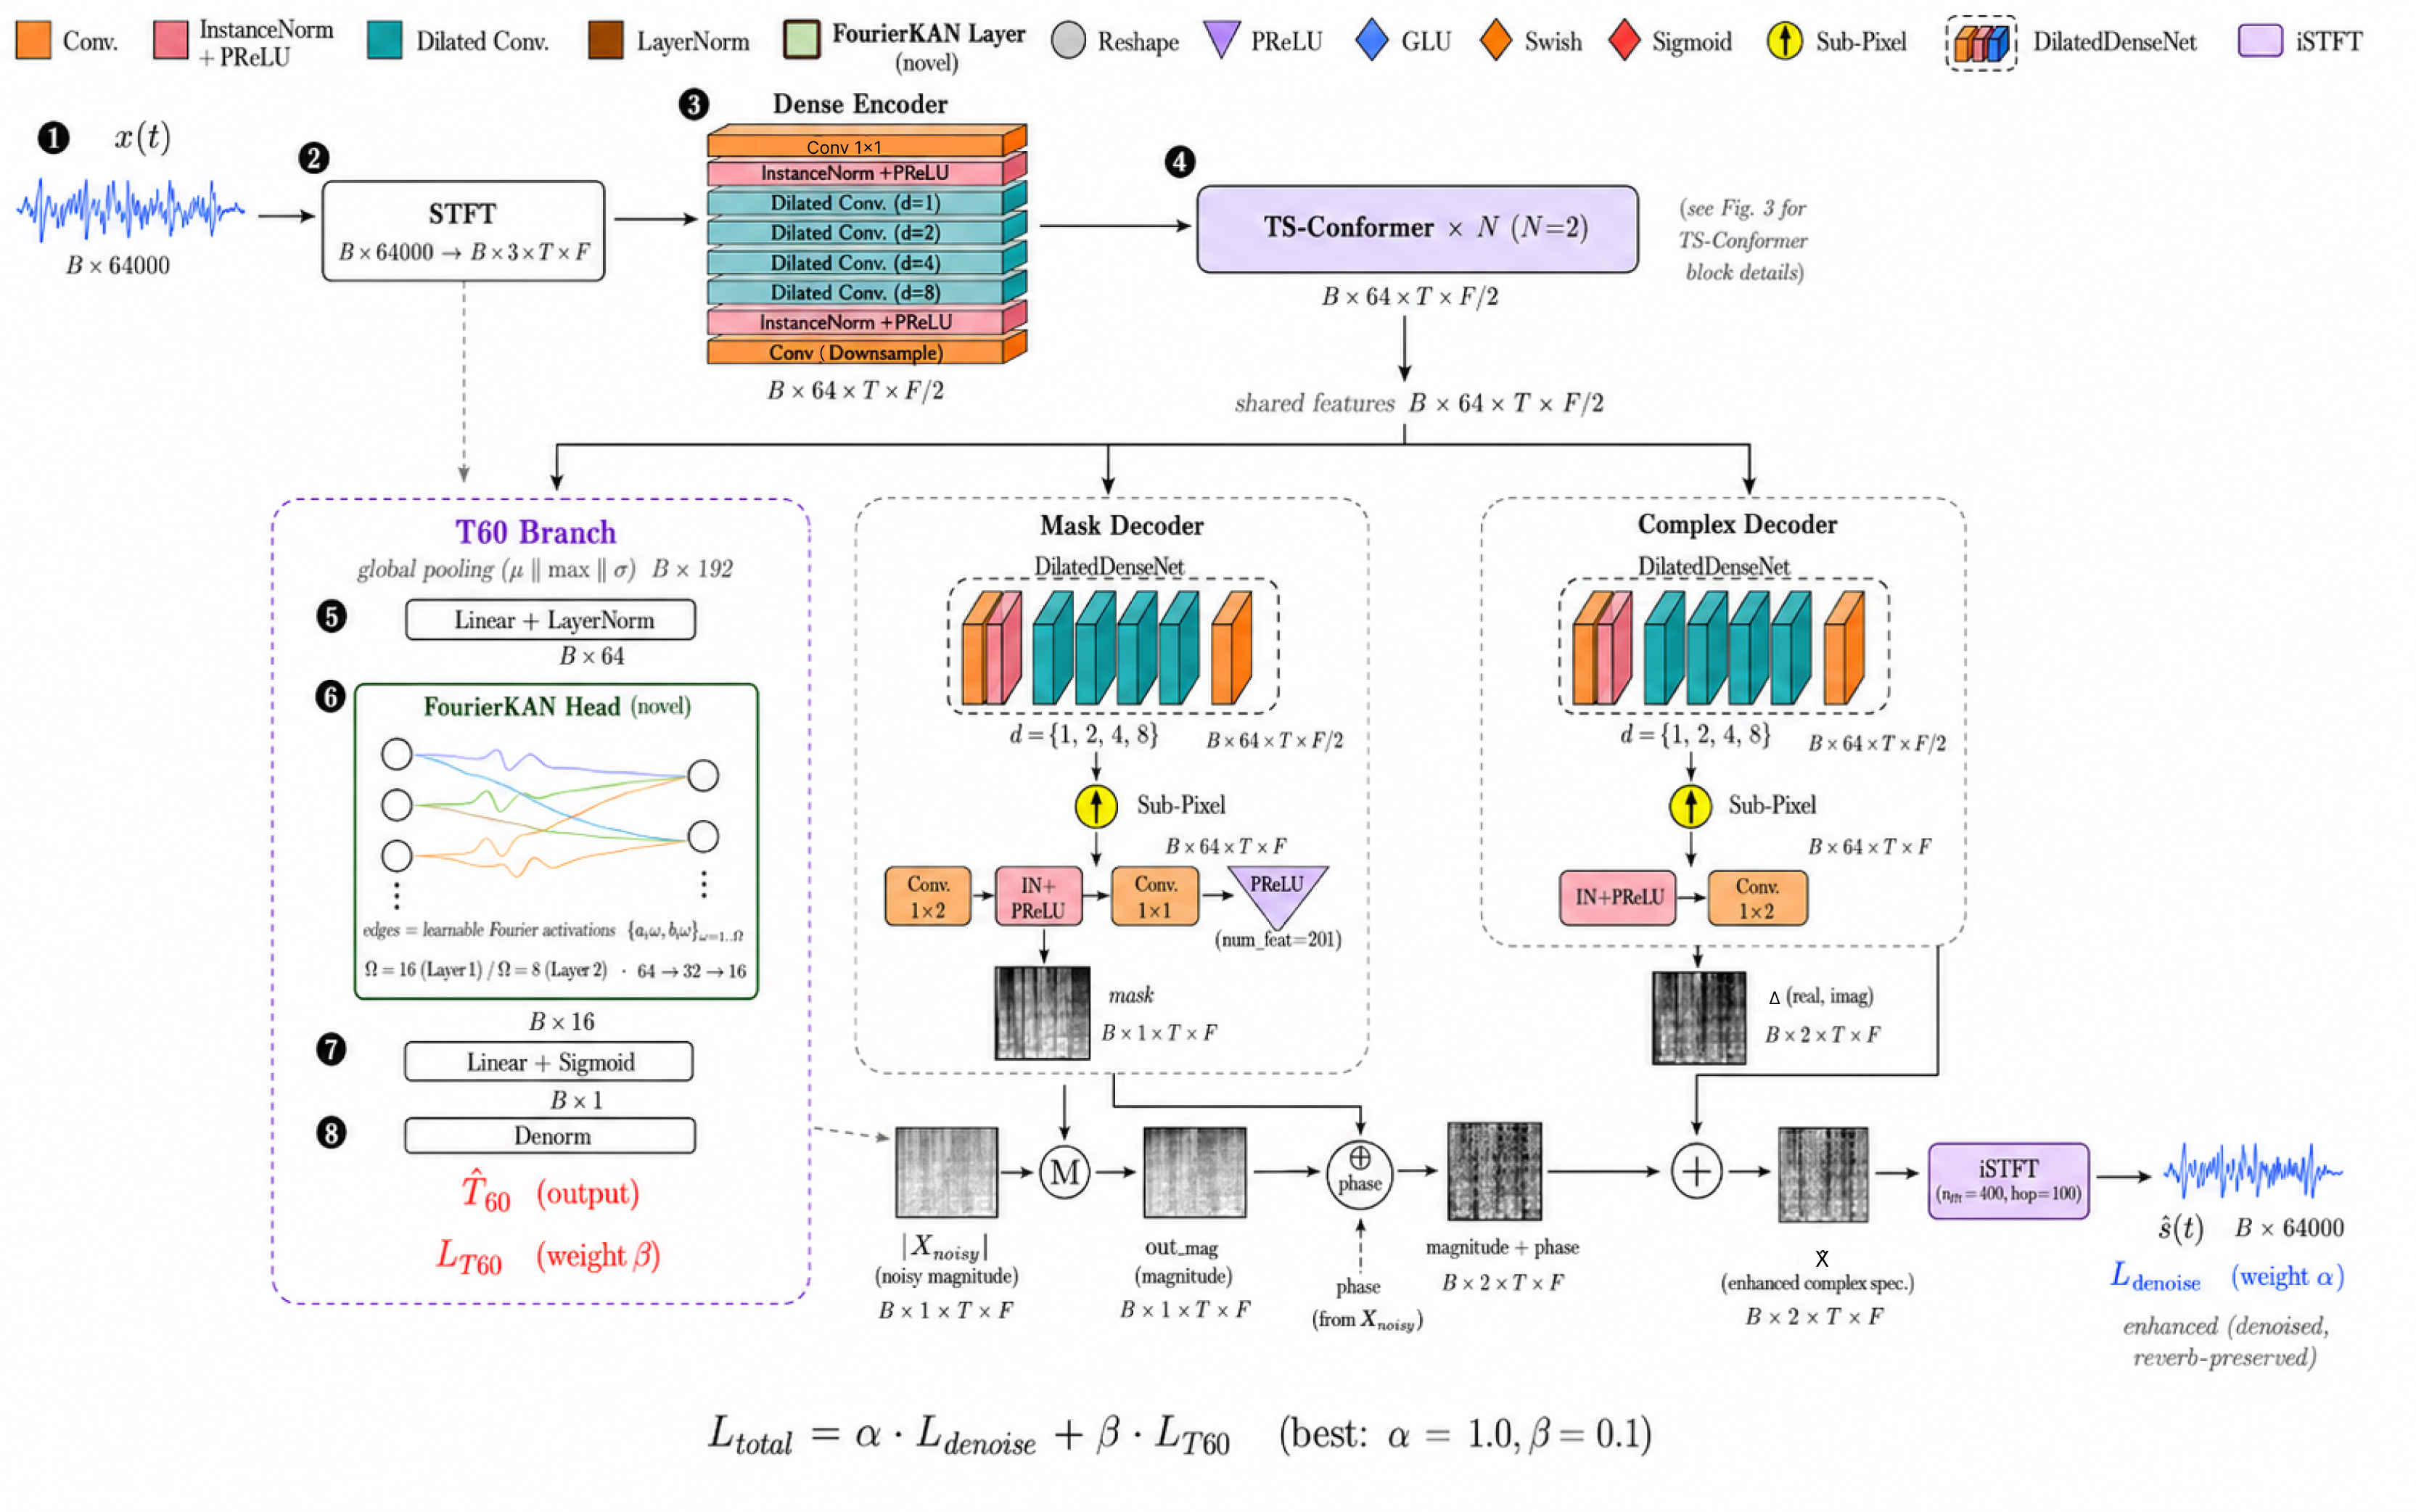
\includegraphics[width=\textwidth]{figs/overall_multitask.png}
  \caption{Overview of the proposed multi-task Conformer-based $T_{60}$
  estimation network. Complex STFT features of the noisy reverberant
  waveform $x(t)$ are processed by a dense convolutional encoder and
  $N{=}2$ stacked two-stage Conformer blocks (TSCBs; see
  Fig.~\ref{fig:tsconformer} for the internal block structure), producing
  a shared bottleneck of shape $B{\times}64{\times}T{\times}F/2$. Three
  branches diverge from the shared bottleneck. The \emph{$T_{60}$ Branch}
  applies channel-wise global statistics pooling
  ($\mu\,\|\,\max\,\|\,\sigma$) followed by a Linear--LayerNorm
  projection, a two-layer Fourier-KAN head ($\Omega{=}16,8$;
  $64{\to}32{\to}16$), a Linear--Sigmoid and an inverse min--max
  denormalisation to yield $\hat{T}_{60}$. The \emph{Mask Decoder} and
  the \emph{Complex Decoder} reuse the CMGAN dilated DenseNet
  ($d\in\{1,2,4,8\}$) and sub-pixel upsampling to predict a real-valued
  magnitude mask and a complex residual $\Delta(\mathrm{real},
  \mathrm{imag})$. Spectral recombination multiplies the mask with the
  noisy magnitude (operator $\mathrm{M}$), reattaches the noisy phase
  $\angle X$ and adds the complex residual ($\oplus$) to obtain the
  reconstructed complex spectrum $\hat{X}$, which is inverted by iSTFT
into the enhanced waveform $\hat{s}(t)$. The two tasks are trained
jointly with the loss
$\mathcal{L}_{\mathrm{total}}=\alpha\,\mathcal{L}_{\mathrm{denoise}}
+\beta\,\mathcal{L}_{T_{60}}$ (the task weights $(\alpha,\beta)$ are
tuned in Section~\ref{sec:res:ablation}); see
Section~\ref{sec:method:loss} for the full definition.}
  \label{fig:overall}
\end{figure*}

\subsection{Dense convolutional encoder}\label{sec:method:encoder}

The dense convolutional encoder turns the noisy reverberant waveform
into a high-dimensional time--frequency representation that is shared
by both tasks. All recordings are resampled to $16$\,kHz, converted to
mono and truncated or padded to a fixed length of $4$\,s, yielding
$L=64\,000$ samples per utterance. To make the input statistics
independent of the absolute recording level, each waveform $y[n]$ is
scaled by an energy-normalising factor
\begin{equation}\label{eq:energy_norm}
  c = \sqrt{\frac{L}{\sum_{n=0}^{L-1} y^{2}[n]+\varepsilon}},\qquad
  \tilde{y}[n] = c\,y[n],
\end{equation}
with $\varepsilon=10^{-8}$ added for numerical stability. The same
normalisation is applied at training and at inference time so that the
network never sees the raw signal level. A complex STFT is then
computed with a Hamming analysis window of $N=400$ samples and a hop
size of $H=100$ samples, yielding a complex spectrum
$\mathbf{Y}\in\mathbb{C}^{T\times F}$ of $T=641$ frames and $F=201$
frequency bins. The real and imaginary parts of $\mathbf{Y}$ are stacked
into a two-channel tensor and the magnitude $|\mathbf{Y}|=
\sqrt{\mathrm{Re}(\mathbf{Y})^{2}+\mathrm{Im}(\mathbf{Y})^{2}}$ is
concatenated as a third channel, producing the input tensor
\begin{equation}\label{eq:input_tensor}
  \mathbf{X}_{\mathrm{in}} = \bigl[\,|\mathbf{Y}|,\;
   \mathrm{Re}(\mathbf{Y}),\;\mathrm{Im}(\mathbf{Y})\,\bigr]
   \in\mathbb{R}^{3\times T\times F}.
\end{equation}
No power-law magnitude compression is applied, as $T_{60}$
depends on the decay shape of the envelope rather than on its
instantaneous loudness.

The encoder uses a dense convolutional design with three stages. A
pointwise convolution first projects the three-channel input to $C=64$
channels and is followed by instance normalisation and a parametric
ReLU. A \emph{dilated dense block} of depth $D=4$ then applies four
cascaded $2\times 3$ convolutions whose inputs are formed by
concatenating the outputs of all preceding convolutions; the dilation
rate of the $d$-th convolution along the time axis is $2^{d-1}$, which
exponentially enlarges the temporal receptive field while keeping the
parameter count under control. Each convolution is followed by an
instance normalisation and a PReLU activation. Finally, a strided
$1\times 3$ convolution downsamples the frequency axis by a factor of
two and produces the encoder bottleneck
\begin{equation}\label{eq:encoder}
  \mathbf{F}^{(0)} = \mathrm{Encoder}(\mathbf{X}_{\mathrm{in}})
        \in \mathbb{R}^{C\times T\times F'},
\end{equation}
with $C=64$, $T=641$ and $F'=101$.

\subsection{Two-stage Conformer block}\label{sec:method:tscb}

The encoder bottleneck $\mathbf{F}^{(0)}$ is further refined by
$N=2$ stacked two-stage Conformer blocks (TSCBs). The Conformer
block~\citep{gulati2020conformer} combines the global modelling
ability of self-attention with the local feature extraction of
convolutions, and has become a standard sequence-modelling choice for
speech enhancement and source separation. For a sequence
$\mathbf{Z}\in\mathbb{R}^{L\times d}$ of length $L$ and feature
dimension $d$, the block consists of four sub-modules wrapped in
residual connections:
\begin{equation}\label{eq:conformer}
  \begin{aligned}
    \mathbf{Z}_1 &= \mathbf{Z} + \tfrac{1}{2}\,\mathrm{FFN}_1(\mathbf{Z}),\\
    \mathbf{Z}_2 &= \mathbf{Z}_1 + \mathrm{MHSA}(\mathbf{Z}_1),\\
    \mathbf{Z}_3 &= \mathbf{Z}_2 + \mathrm{Conv}(\mathbf{Z}_2),\\
    \mathbf{Z}_4 &= \mathrm{LayerNorm}\bigl(\mathbf{Z}_3 +
                    \tfrac{1}{2}\,\mathrm{FFN}_2(\mathbf{Z}_3)\bigr),
  \end{aligned}
\end{equation}
where $\mathrm{FFN}_1$ and $\mathrm{FFN}_2$ are two pre-normalised
position-wise feed-forward modules with Swish activations,
$\mathrm{MHSA}$ is a multi-head self-attention module with Shaw-style
relative positional encoding~\citep{shaw2018relativepos}, and
$\mathrm{Conv}$ is a depth-wise separable 1-D convolution module with a
gated linear unit and a batch normalisation. The half-scaling of the two
feed-forward branches yields the so-called ``Macaron'' structure that
has been shown to stabilise optimisation~\citep{gulati2020conformer}.

When applied to a time--frequency representation of speech, the
Conformer block is typically deployed in a dual-path fashion: two
Conformer blocks are stacked, one operating along the time axis and one
along the frequency axis, jointly forming a two-stage Conformer block
(TSCB)~\citep{cao2022cmgan}. Concretely, for an input feature map
$\mathbf{F}\in\mathbb{R}^{B\times C\times T\times F'}$:
\begin{equation}\label{eq:tscb_time}
  \mathbf{F}^{t} = \mathbf{F}
      + \mathrm{ConformerBlock}_{t}\bigl(\mathrm{Reshape}_{t}(\mathbf{F})\bigr),
\end{equation}
where $\mathrm{Reshape}_{t}$ flattens the frequency axis into the batch
dimension and treats the time axis as the sequence axis; the Conformer
block then operates on tensors of shape $(B\,F')\times T\times C$.
Analogously,
\begin{equation}\label{eq:tscb_freq}
  \mathbf{F}^{tf} = \mathbf{F}^{t}
      + \mathrm{ConformerBlock}_{f}\bigl(\mathrm{Reshape}_{f}(\mathbf{F}^{t})\bigr),
\end{equation}
with $\mathrm{Reshape}_{f}$ producing tensors of shape $(B\,T)\times
F'\times C$. Each Conformer block has $h=4$ attention heads of dimension
$d_h=C/4=16$, a feed-forward expansion factor of $4$, a depth-wise
separable 1-D convolution with kernel size $31$, and a dropout rate of
$0.2$ on both the attention and the feed-forward sub-modules. After
the second TSCB, the bottleneck feature map is denoted
$\mathbf{F}^{(N)}\in\mathbb{R}^{C\times T\times F'}$. With $C=64$,
$T=641$ and $F'=101$, the per-block self-attention has quadratic
complexity in $T$ or $F'$ but only linear complexity in the product
$T\,F'$ thanks to the dual-path factorisation; this is what makes a
$4$-second window tractable on a single GPU. The resulting bottleneck
$\mathbf{F}^{(N)}$ is shared by both the $T_{60}$ regression head
(Section~\ref{sec:method:head}) and the denoising branch
(Section~\ref{sec:method:denoise}).

\begin{figure}[H]
  \centering
  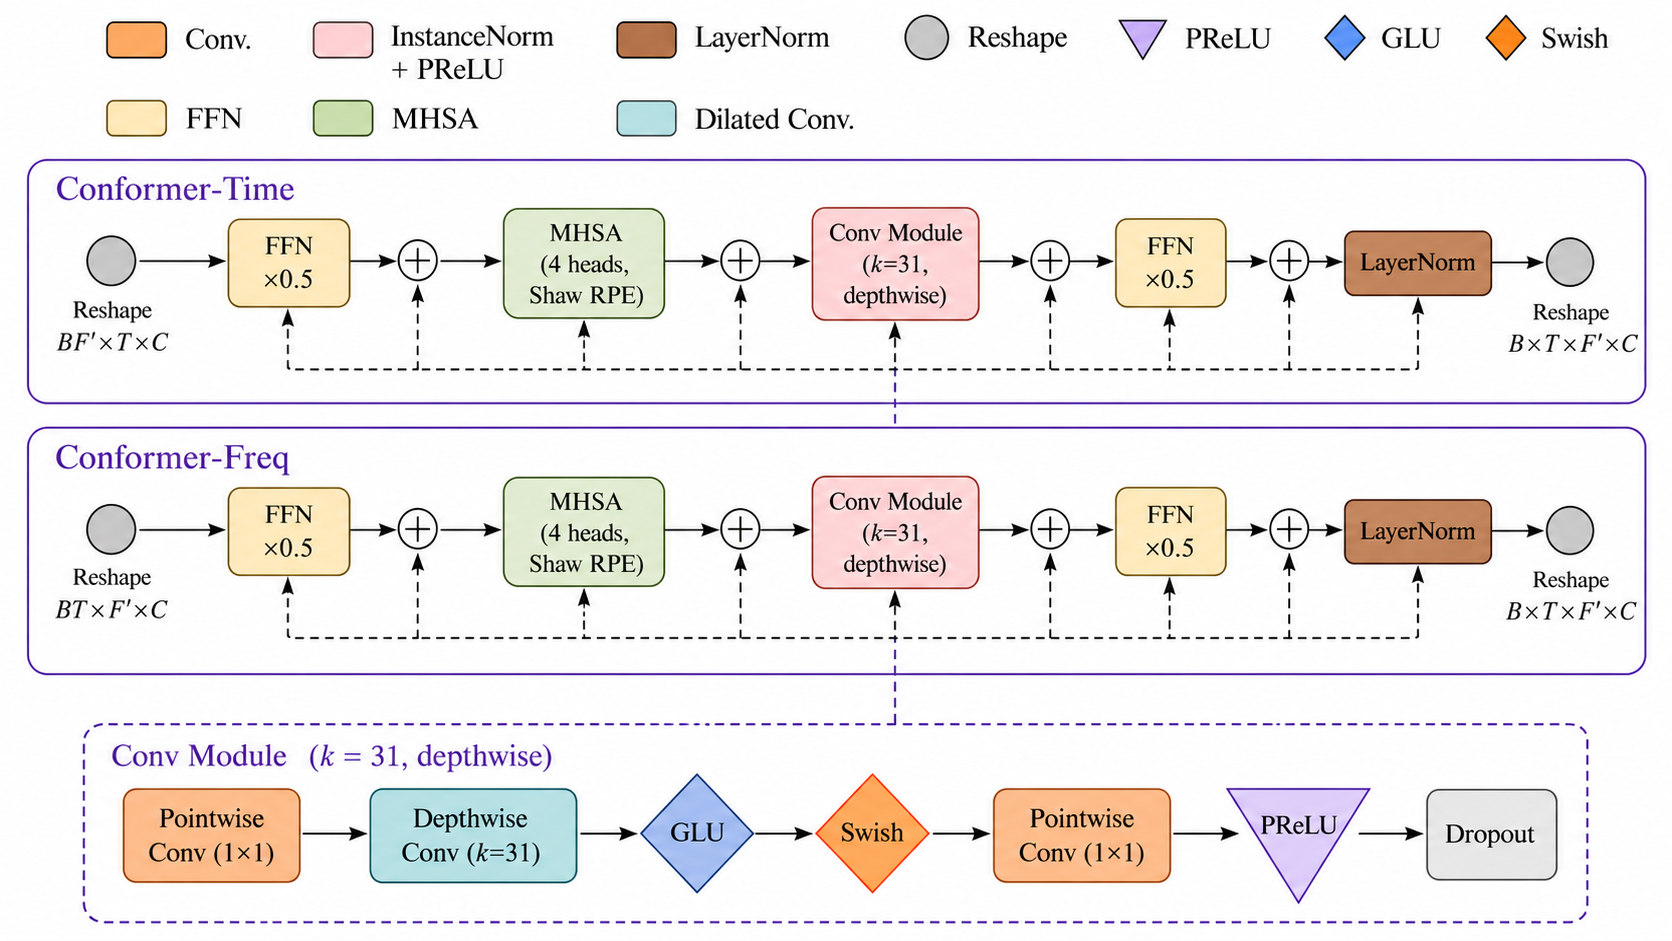
\includegraphics[width=\columnwidth]{figs/tsconformer_block.png}
  \caption{Internal structure of a two-stage Conformer block (TSCB)
  used in the shared backbone of Fig.~\ref{fig:overall}. The block is the
  serial composition of a time-axis Conformer (Conformer-Time, input
  shape $BF'{\times}T{\times}C$), a frequency-axis Conformer
  (Conformer-Freq, input shape $BT{\times}F'{\times}C$) and a final
  reshape back to $B{\times}T{\times}F'{\times}C$. Each Conformer
  variant follows the Macaron design: two half-step feed-forward
  modules sandwich a multi-head self-attention (MHSA, $h{=}4$, Shaw
  relative positional encoding) and a depth-wise separable convolution
  module (Conv Module, kernel size $k{=}31$), all wrapped in residual
  connections ($\oplus$). The dashed arrow expands the inner structure
  of the Conv Module into a pointwise-conv $\to$ depthwise-conv $\to$
  GLU $\to$ Swish $\to$ pointwise-conv $\to$ PReLU $\to$ dropout
  pipeline.}
  \label{fig:tsconformer}
\end{figure}

\subsection{$T_{60}$ regression head}\label{sec:method:head}

The $T_{60}$ regression head condenses the shared bottleneck
$\mathbf{F}^{(N)}$ into a single normalised $T_{60}$ estimate through
two-step pooling followed by a Fourier-KAN block. The frequency axis is
first averaged, which reflects the assumption that $T_{60}$ summarises a
broadband property of the room rather than a specific spectral pattern:
\begin{equation}\label{eq:freq_avg}
  \mathbf{Z}_{c,t} = \frac{1}{F'}\sum_{f=1}^{F'}\mathbf{F}^{(N)}_{c,t,f},
\end{equation}
yielding $\mathbf{Z}\in\mathbb{R}^{C\times T}$. The time axis is then
aggregated by a multi-statistic pooling layer that computes the average,
the maximum and the standard deviation along the time
dimension~\citep{snyder2018xvector}:
\begin{equation}\label{eq:multipool}
  \mathbf{e} = \bigl[\,\mu(\mathbf{Z}),\;
   \max(\mathbf{Z}),\;\sigma(\mathbf{Z})\,\bigr] \in \mathbb{R}^{3C}.
\end{equation}
The three statistics carry complementary information about the energy
envelope of the utterance: $\mu(\mathbf{Z})$ summarises the long-term
average level, $\max(\mathbf{Z})$ captures the peak excitation typically
associated with vowel onsets, and $\sigma(\mathbf{Z})$ captures the
temporal modulation of the envelope, which is known to be strongly
correlated with the decay rate of the late reverberation
tail~\citep{falk2010temporal}. With $C=64$, the resulting embedding has
$3C=192$ entries.

\paragraph{Kolmogorov--Arnold basis.} The Kolmogorov--Arnold representation theorem states that any
continuous multivariate function $f:[0,1]^{n}\to\mathbb{R}$ can be
written as the finite composition of univariate continuous functions
and addition. \citet{liu2024kan} build on this observation and propose
Kolmogorov--Arnold networks (KANs), in which the fixed scalar
non-linearities of a multi-layer perceptron (MLP) are replaced by
learnable univariate functions placed on every \emph{edge} of the
network. A single KAN layer with input dimension $I$ and output
dimension $O$ implements the mapping
\begin{equation}\label{eq:kan_layer}
  y_j = \sum_{i=1}^{I} \phi_{j,i}(x_i) + b_j,
  \qquad j=1,\ldots,O,
\end{equation}
where each $\phi_{j,i}:\mathbb{R}\to\mathbb{R}$ is a learnable univariate
function and $b_j$ is a per-output bias. The original KAN paper
parameterises $\phi_{j,i}$ by cubic B-splines, which is expressive but
requires bookkeeping such as adaptive grid updates and is comparatively
slow on small batch sizes typical of regression heads.

A Fourier-KAN replaces the spline basis by a truncated trigonometric
series~\citep{xu2025fourierkan}. For a
\emph{frequency count} $\Omega\in\mathbb{N}$, every edge function is
written as
\begin{equation}\label{eq:fourier_phi}
  \phi_{j,i}(x_i) = \sum_{\omega=1}^{\Omega}
    \bigl[a_{j,i,\omega}\,\cos(\omega\,x_i)
        + b_{j,i,\omega}\,\sin(\omega\,x_i)\bigr],
\end{equation}
so that the output of a Fourier-KAN layer becomes
\begin{equation}\label{eq:fourier_layer}
  y_j = \sum_{i=1}^{I}\sum_{\omega=1}^{\Omega}
        \bigl[a_{j,i,\omega}\cos(\omega x_i)
            + b_{j,i,\omega}\sin(\omega x_i)\bigr] + b_j.
\end{equation}
The number of trainable parameters per layer is $2\,O\,I\,\Omega + O$,
which is a modest multiple of an equivalent linear layer of size
$O\times I$ but still small in absolute terms when $I$ and $O$ are kept
small. Two properties make this basis attractive for the proposed
regression head: (i) gradients with respect to the weights are
closed-form trigonometric functions of the input and require no grid
maintenance; (ii) the basis has a strong inductive bias towards smooth
and approximately periodic dependencies, which matches the empirical
shape of the mapping from pooled bottleneck statistics to $T_{60}$.

The pooled embedding $\mathbf{e}\in\mathbb{R}^{192}$ is mapped to the
final estimate $\hat{T}_{60}$ by the Fourier-KAN head, depicted
in Fig.~\ref{fig:head}. The head is composed of a linear
projection, a stack of two Fourier-KAN layers and a final linear output.
Each step is described below.

\paragraph{Projection.} A linear projection followed by a layer
normalisation reduces the pooled embedding to a $d_{0}=64$-dimensional
vector,
\begin{equation}\label{eq:proj}
  \mathbf{u}^{(0)} = \mathrm{LayerNorm}\bigl(\mathbf{W}_{p}\,\mathbf{e}+
                                              \mathbf{b}_{p}\bigr),
  \qquad \mathbf{u}^{(0)}\in\mathbb{R}^{d_{0}}.
\end{equation}
No additional activation is applied after the layer normalisation:
the normalisation already constrains the input range of the first
Fourier layer, and a saturating non-linearity such as tanh would reduce
the effective capacity of the periodic basis.

\paragraph{Fourier-KAN block.} The projected embedding is processed by
$L=2$ Fourier-KAN layers with hidden dimensions $(d_{1},d_{2})=(32,16)$.
The first layer uses a comparatively large frequency count
$\Omega_{0}=16$, which allows it to learn fine-grained non-linear
features directly from the embedding, while the inner layer uses a
smaller budget $\Omega_{1}=8$ for parameter efficiency. Formally, for
$\ell=1,2$,
\begin{equation}\label{eq:fourier_block}
  u^{(\ell)}_j = \sum_{i=1}^{d_{\ell-1}}\sum_{\omega=1}^{\Omega_{\ell-1}}
    \bigl[a^{(\ell)}_{j,i,\omega}\cos(\omega u^{(\ell-1)}_i)
        + b^{(\ell)}_{j,i,\omega}\sin(\omega u^{(\ell-1)}_i)\bigr]
    + c^{(\ell)}_j,
\end{equation}
and the layer output is post-processed by a layer normalisation and a
dropout with probability $0.1$:
\begin{equation}\label{eq:fourier_post}
  \mathbf{u}^{(\ell)} \leftarrow \mathrm{Dropout}\bigl(
    \mathrm{LayerNorm}(\mathbf{u}^{(\ell)})\bigr).
\end{equation}
The Fourier weights $a^{(\ell)}_{j,i,\omega}$ and $b^{(\ell)}_{j,i,\omega}$
are initialised from a zero-mean Gaussian with standard deviation
$\sqrt{1/(d_{\ell-1}\,\Omega_{\ell-1})}$, so that the variance of the
layer output is approximately unity at initialisation regardless of the
input dimension and the frequency count.

\paragraph{Output.} A linear layer maps $\mathbf{u}^{(2)}\in
\mathbb{R}^{16}$ to a scalar, and a sigmoid activation produces the
normalised estimate
\begin{equation}\label{eq:t60_hat}
  \hat{T}_{60}^{\mathrm{norm}} = \sigma\bigl(\mathbf{w}_{o}^{\top}\mathbf{u}^{(2)}
                                            + b_{o}\bigr) \in (0,1).
\end{equation}

\subsection{Denoising decoder branch}\label{sec:method:denoise}

To inject denoising supervision into the shared backbone, a decoder
branch is tapped off the bottleneck feature $\mathbf{F}^{(N)}$ using the
mask-plus-complex-residual structure of CMGAN~\citep{cao2022cmgan}. A
mask decoder outputs a magnitude mask
$\mathbf{M}\in\mathbb{R}^{1\times T\times F}$, multiplied with the input
magnitude to give the masked magnitude
$\hat{M}=|\mathbf{Y}|\odot\mathbf{M}$, while a complex decoder outputs a
complex residual $\Delta\in\mathbb{R}^{2\times T\times F}$. Combined
with the noisy phase $\angle\mathbf{Y}$, the real and imaginary parts of
the enhanced spectrum are reconstructed as
\begin{equation}\label{eq:denoise_branch}
  \hat{Y}_{\mathrm{re}} = \hat{M}\cos(\angle\mathbf{Y}) + \Delta_{\mathrm{re}},\qquad
  \hat{Y}_{\mathrm{im}} = \hat{M}\sin(\angle\mathbf{Y}) + \Delta_{\mathrm{im}},
\end{equation}
and an inverse STFT yields the enhanced time-domain speech. Both
decoders adopt a dense design mirroring the encoder. The denoising
target is the clean reverberant speech $\tilde{s}(t)=s(t)\ast h(t)$,
i.e.\ the noise-free reverberant component of
Eq.~\eqref{eq:time_model}, so this branch performs denoising rather than
dereverberation---the enhanced speech still carries the room
reverberation.

\subsection{Loss function}\label{sec:method:loss}

To match the output range of the sigmoid in Eq.~\eqref{eq:t60_hat},
every ground-truth $T_{60}$ value is linearly mapped to $[0,1]$ before
being fed to the loss function:
\begin{equation}\label{eq:t60_norm}
  T_{60}^{\mathrm{norm}}
  = \frac{T_{60} - T_{\min}}{T_{\max} - T_{\min}}.
\end{equation}
The $T_{60}$ regression loss is the mean squared error between the
predicted and the ground-truth normalised $T_{60}$ on a mini-batch of
$B$ utterances,
\begin{equation}\label{eq:t60_loss}
  \mathcal{L}_{T_{60}}(\boldsymbol{\theta})
  = \frac{1}{B}\sum_{i=1}^{B}\bigl(\hat{T}_{60,i}^{\mathrm{norm}}
                                  - T_{60,i}^{\mathrm{norm}}\bigr)^{2}.
\end{equation}
The denoising loss combines a compressed-domain real/imaginary loss, a
magnitude loss and a time-domain loss,
\begin{equation}\label{eq:denoise_loss}
  \mathcal{L}_{\mathrm{den}}
  = w_{ri}\,\mathcal{L}_{ri} + w_{mag}\,\mathcal{L}_{mag}
    + w_{time}\,\mathcal{L}_{time},
\end{equation}
where $\mathcal{L}_{ri}$ and $\mathcal{L}_{mag}$ are mean-squared errors
on the (power-compressed) real/imaginary parts and magnitude of the
enhanced spectrum against the clean reverberant target $\tilde{S}$, and
$\mathcal{L}_{time}$ is an $\ell_{1}$ loss between the inverse-STFT
enhanced waveform and $\tilde{s}$. As the raw denoising and $T_{60}$
losses differ in scale, each is first divided by its own exponential
moving average (EMA) to bring $\mathcal{L}_{\mathrm{den}}^{*}$ and
$\mathcal{L}_{T_{60}}^{*}$ to a common scale, so that the two losses
can be weighted on a single dimension; the two tasks are then optimised
jointly through the weighted sum
\begin{equation}\label{eq:loss}
  \mathcal{L}(\boldsymbol{\theta})
  = \alpha\,\mathcal{L}_{\mathrm{den}}^{*}(\boldsymbol{\theta})
    + \beta\,\mathcal{L}_{T_{60}}^{*}(\boldsymbol{\theta}),
\end{equation}
where $\boldsymbol{\theta}$ collects all trainable parameters of the
shared encoder and TSCBs, the Fourier-KAN head and the two denoising
decoders; the denoising sub-weights are
$(w_{ri},w_{mag},w_{time})=(0.1,0.9,0.2)$. The specific values of
$(\alpha,\beta)$ and the corresponding main-model configuration are
given in Section~\ref{sec:exp:impl}.

At inference time the sigmoid output is denormalised by the inverse of
Eq.~\eqref{eq:t60_norm} to yield the final estimate
$\hat{T}_{60}\in[T_{\min}, T_{\max}]$.

% =====================================================================
\section{Experiments}\label{sec:exp}
% =====================================================================

\subsection{Dataset}\label{sec:exp:data}

Experiments are conducted on the T60\_Dataset\_v7\_4s dataset, which
consists of $16$\,kHz mono noisy reverberant speech clips of about
$4$\,s. Each sample directory
\texttt{speech\{id\}\_reverb\_\{T60\}\_\{SNR\}dB/} contains three files:
the noisy reverberant recording \texttt{\{name\}.wav} (model input), the
noise-free reverberant speech \texttt{\{name\}\_denoised.wav} (denoising
target), and the noise component \texttt{\{name\}\_noise.wav} (unused).
$T_{60}$ covers $[0.1, 1.5]$\,s and the SNR covers $-5$ to $20$\,dB. The
dataset is split into a training set of $40\,000$ clips, a validation
set of $5\,136$ clips, and four test sets of $1\,080$ clips each, forming
a $2\times 2$ design over simulated/real RIRs and seen/unseen noise
(Table~\ref{tab:testsets}). ``Seen/unseen'' refers to whether the noise
type appears in the training set; this design evaluates robustness to
RIR realism and to noise generalisation. Figure~\ref{fig:dataset} shows
the $T_{60}$ distribution of the training pool and of the test sets
(grouped by RIR type).

\begin{figure}[H]
  \centering
  \begin{minipage}[t]{0.48\textwidth}
    \centering
    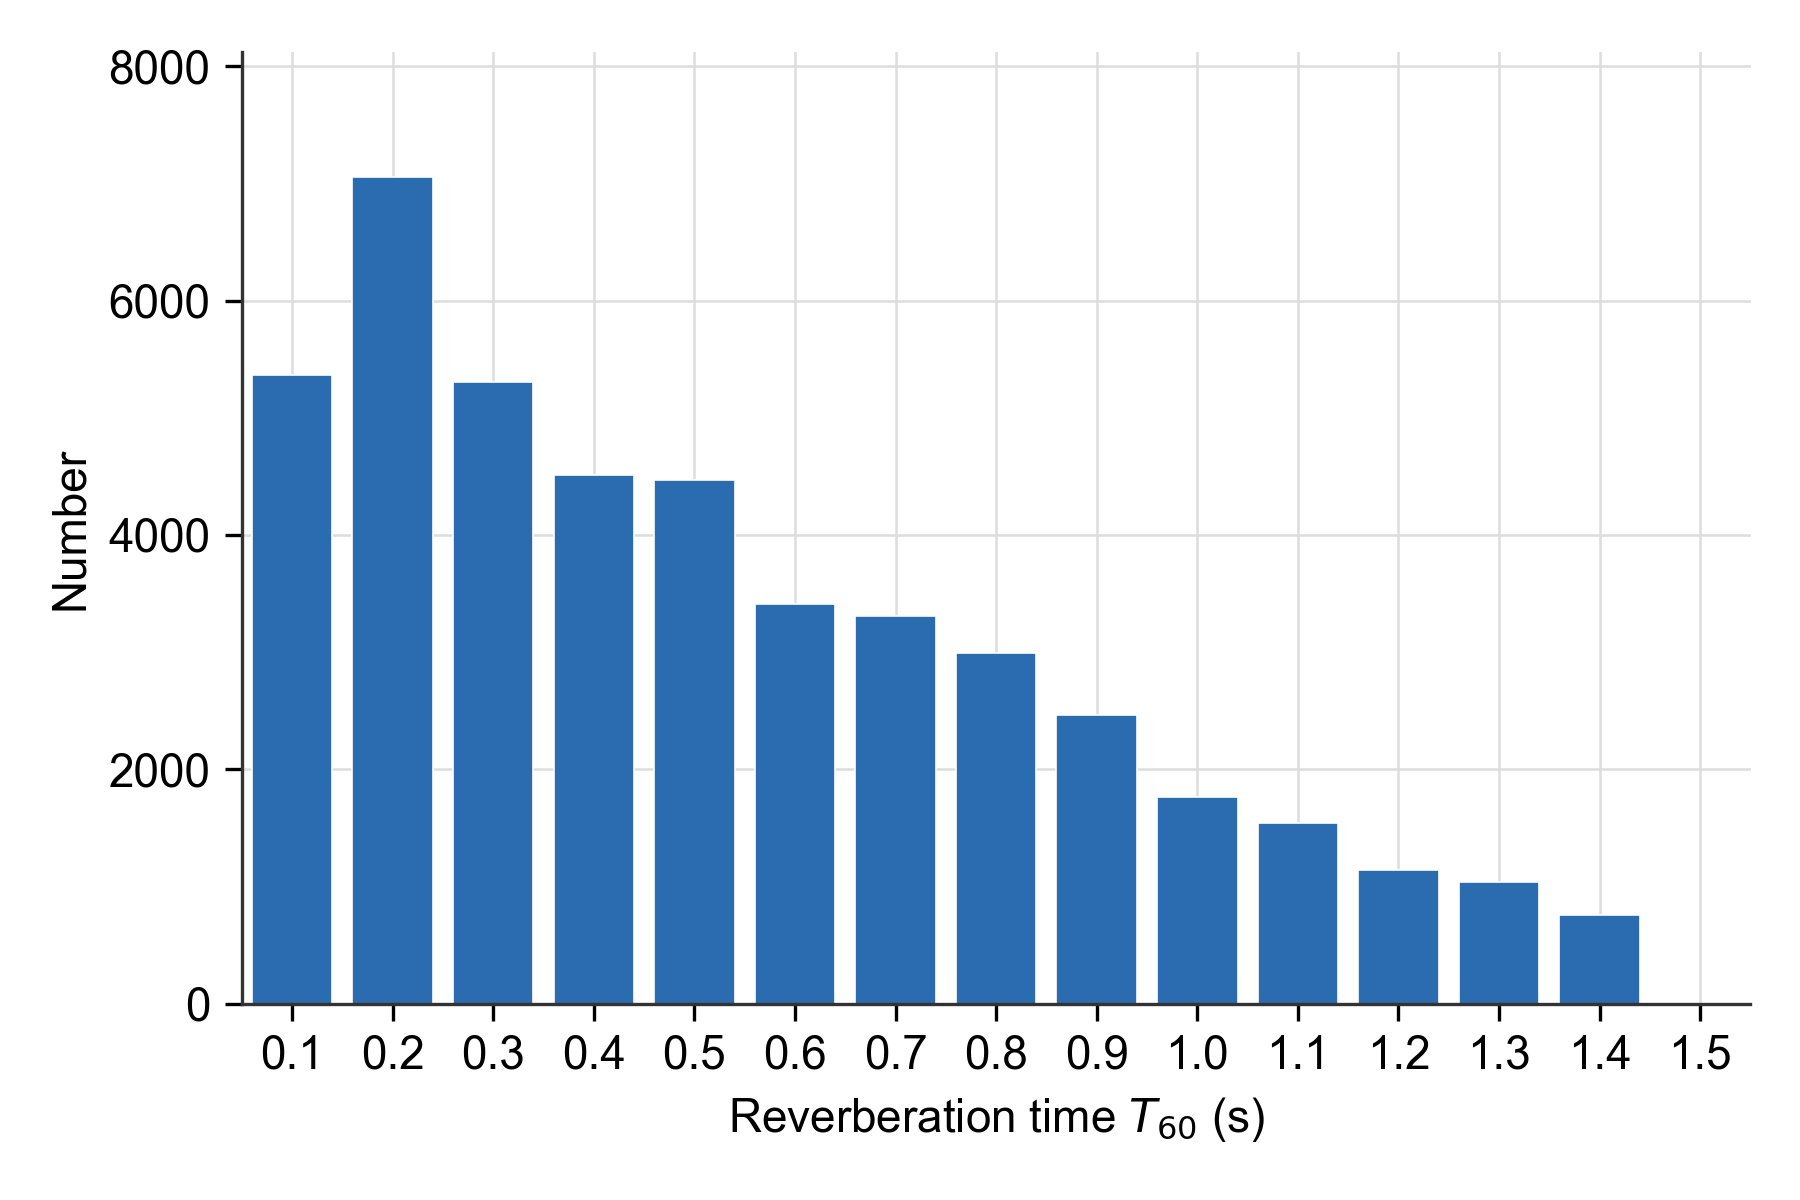
\includegraphics[width=\linewidth]{figs/dataset_distribution_train.png}\\[2pt]
    {\small (a) Training pool.}
  \end{minipage}\hfill
  \begin{minipage}[t]{0.48\textwidth}
    \centering
    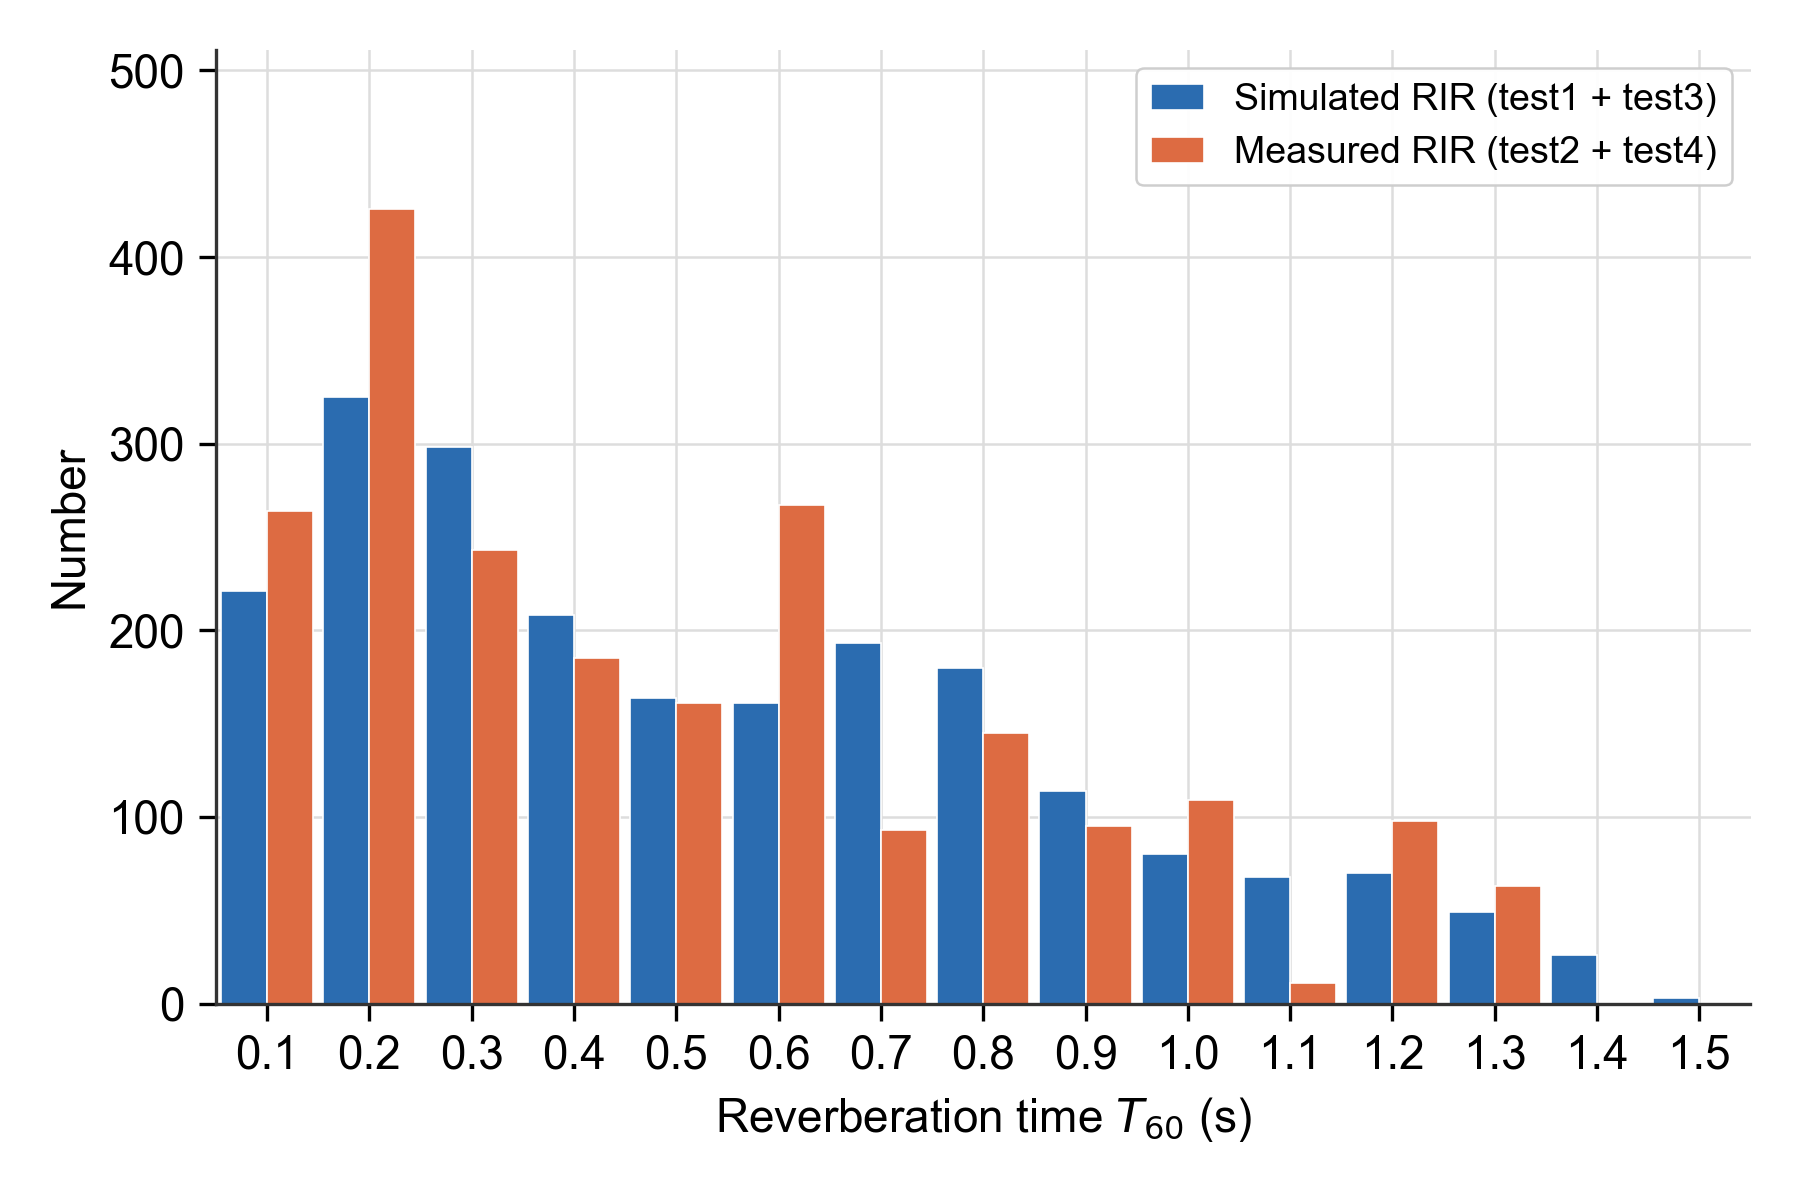
\includegraphics[width=\linewidth]{figs/dataset_distribution_test.png}\\[2pt]
    {\small (b) Test sets: simulated RIRs vs.\ real RIRs.}
  \end{minipage}
  \caption{$T_{60}$ distribution of dataset.}
  \label{fig:dataset}
\end{figure}

\begin{table}[!htbp]
  \centering
  \caption{Test-set design: simulated vs.\ real RIR $\times$ seen vs.\
  unseen noise.}
  \label{tab:testsets}
  \begin{tabular}{lll}
    \toprule
    Test set & RIR & Noise \\
    \midrule
    test1 & simulated (image-source) & seen \\
    test2 & real (measured)          & seen \\
    test3 & simulated (image-source) & unseen \\
    test4 & real (measured)          & unseen \\
    \bottomrule
  \end{tabular}
\end{table}

\subsection{Baselines and metrics}\label{sec:exp:baselines}

\paragraph{Baselines.} The proposed model is compared with three blind
$T_{60}$ estimators on the same dataset: (i) BERP
\citep{wang2025berp}, a universal blind room-parameter estimator with an
attention-and-convolution unified encoder and separate per-parameter
predictors; (ii) DAMTL \citep{zhang2024damtl}, a denoising-aided
multi-task $T_{60}$ estimator; and (iii) the noise-aware time--frequency
masking method \citep{zheng2022noiseaware}, a two-stage framework. All
three are re-trained and evaluated on T60\_Dataset\_v7 with the same
splits for a fair comparison.

\paragraph{Evaluation metrics.}

$T_{60}$ estimation accuracy and denoising quality are evaluated with
the following metrics.

\paragraph{$T_{60}$ estimation.}
\begin{description}
  \item[Root-mean-squared error (RMSE).] The standard deviation of the
  estimation residuals,
  \begin{equation}\label{eq:rmse}
    \mathrm{RMSE}=\sqrt{\frac{1}{N}\sum_{i=1}^{N}(\hat{T}_{60,i}-T_{60,i})^{2}},
  \end{equation}
  which penalises large errors more heavily; lower is better. $T_{60}$
  values are reported in milliseconds.
  \item[Mean absolute error (MAE).] The average absolute deviation,
  \begin{equation}\label{eq:mae}
    \mathrm{MAE}=\frac{1}{N}\sum_{i=1}^{N}|\hat{T}_{60,i}-T_{60,i}|,
  \end{equation}
  an error measure on the same scale as $T_{60}$; lower is better.
  \item[Pearson correlation coefficient ($r$).] The linear correlation
  between estimates and ground truth,
  \begin{equation}\label{eq:pearson}
    r=\frac{\sum_{i}(\hat{T}_{60,i}-\bar{\hat{T}}_{60})(T_{60,i}-\bar{T}_{60})}{\sqrt{\sum_{i}(\hat{T}_{60,i}-\bar{\hat{T}}_{60})^{2}}\sqrt{\sum_{i}(T_{60,i}-\bar{T}_{60})^{2}}},
  \end{equation}
  ranging in $[-1,1]$; closer to $1$ is better.
  \item[Coefficient of determination ($R^{2}$).] The proportion of
  variance in $T_{60}$ explained by the estimates,
  \begin{equation}\label{eq:r2}
    R^{2}=1-\frac{\sum_{i}(\hat{T}_{60,i}-T_{60,i})^{2}}{\sum_{i}(T_{60,i}-\bar{T}_{60})^{2}},
  \end{equation}
  ranging in $(-\infty,1]$; closer to $1$ is better.
\end{description}
In addition to the overall metrics, RMSE and $r$ are reported per
$T_{60}$ bin ($0.1$\,s steps) and per SNR bin.

\paragraph{Denoising.}
\begin{description}
  \item[PESQ.] The wide-band perceptual evaluation of speech quality
  (ITU-T P.862.2), scoring $-0.5$ to $4.5$; higher is better.
  \item[STOI.] The short-time objective intelligibility, a $0$--$1$
  measure of speech intelligibility; higher is better.
  \item[SI-SDR.] The scale-invariant signal-to-distortion ratio,
  \begin{equation}\label{eq:sisdr}
    \mathrm{SI\text{-}SDR}=10\log_{10}\frac{\lVert\mathbf{s}_{\mathrm{target}}\rVert^{2}}{\lVert\mathbf{e}_{\mathrm{noise}}\rVert^{2}},
  \end{equation}
  measuring reconstruction fidelity in dB; higher is better.
\end{description}
All denoising metrics are computed on both the noisy input and the
enhanced output and the gains are reported. As noted in
Section~\ref{sec:method:denoise}, the denoising target is the noise-free
reverberant speech, so these metrics measure denoising rather than
dereverberation quality.

\subsection{Model and training setup}\label{sec:exp:impl}

The model architecture is detailed in Section~\ref{sec:method} (shared
DenseEncoder + two TSCBs + Fourier-KAN regression head + CMGAN denoising
decoders); here we only describe the training configuration. All
recordings are resampled to $16$\,kHz mono and chunked/padded to $4$\,s.
We use the AdamW optimiser (learning rate $5\times10^{-4}$, weight decay
$10^{-5}$), batch size $16$, gradient clipping $5.0$, and
mixed-precision training for at most $100$ epochs, with early stopping
when the validation RMSE does not improve for $15$ epochs. Following
Section~\ref{sec:method:loss}, the denoising and $T_{60}$ losses are
each divided by their own EMA to a common scale and combined as
$\mathcal{L}=\alpha\,\mathcal{L}_{\mathrm{den}}^{*}+
\beta\,\mathcal{L}_{T_{60}}^{*}$; the task weights $(\alpha,\beta)$ are
tuned in Section~\ref{sec:res:ablation}.

To check whether the two tasks interfere on the shared layers, every
$20$ training steps and before the main backward pass we measure the
gradients of the two (normalised but unweighted) losses with respect to
the three shared modules (DenseEncoder, TSCB$_{1}$, TSCB$_{2}$) and
record the cosine similarity $\cos$ between them.

% =====================================================================
\section{Results and discussion}\label{sec:results}
% =====================================================================

\subsection{Ablation study}\label{sec:res:ablation}

\paragraph{Task-weight tuning.} We first tune the task weights
$(\alpha,\beta)$ of the normalised loss
$\mathcal{L}=\alpha\,\mathcal{L}_{\mathrm{den}}^{*}+
\beta\,\mathcal{L}_{T_{60}}^{*}$. Table~\ref{tab:weight} reports the
$T_{60}$ accuracy for five configurations spanning the
denoise-dominant, balanced and $T_{60}$-dominant regimes. Accuracy
improves as the denoising weight is increased relative to
the $T_{60}$ weight, and the best result is obtained at
$(\alpha,\beta)=(1.0,0.05)$ with an RMSE of $92.91$\,ms---we therefore
adopt this configuration as the main model throughout the paper. Once
the denoising weight is reduced to the balanced or $T_{60}$-dominant
regime the RMSE deteriorates to $\sim$$110$\,ms, no better than the
single-task baseline ($111.15$\,ms), confirming that accuracy improves
only when the denoising task is given a clearly larger weight.

\begin{table}[!htbp]
  \centering
  \caption{Task-weight ablation (normalised losses; average over
  test1--test4). $T_{60}$ accuracy improves as the denoising weight
  $\alpha/\beta$ increases, with $(1.0,0.05)$ the best.}
  \label{tab:weight}
  \begin{tabular}{lccc}
    \toprule
    Configuration & $(\alpha,\beta)$ & RMSE (ms) $\downarrow$ & MAE (ms) $\downarrow$ \\
    \midrule
    Denoise-dominant (proposed) & (1.0, 0.05) & \textbf{92.91}  & \textbf{56.68} \\
    Denoise-dominant            & (1.0, 0.1)  & 97.79           & 57.95 \\
    Denoise-dominant            & (1.0, 0.3)  & 107.10          & 64.28 \\
    Balanced                    & (1.0, 1.0)  & 109.90          & 67.16 \\
    $T_{60}$-dominant           & (0.1, 1.0)  & 109.54          & 68.15 \\
    \bottomrule
  \end{tabular}
\end{table}

\paragraph{Regression-head ablation.} We further compare the Fourier-KAN
regression head against an MLP head of comparable capacity, both under
the same multi-task configuration $(\alpha,\beta)=(1.0,0.05)$.

\begin{table}[!htbp]
  \centering
  \caption{Regression-head ablation under the multi-task setting
  $(\alpha,\beta)=(1.0,0.05)$.}
  \label{tab:head}
  \begin{tabular}{lcc}
    \toprule
    Head & RMSE (ms) $\downarrow$ & MAE (ms) $\downarrow$ \\
    \midrule
    MLP          & 102.17 & 64.94 \\
    Fourier-KAN  & \textbf{92.91}    & \textbf{56.68} \\
    \bottomrule
  \end{tabular}
\end{table}

\begin{figure}[H]
  \centering
  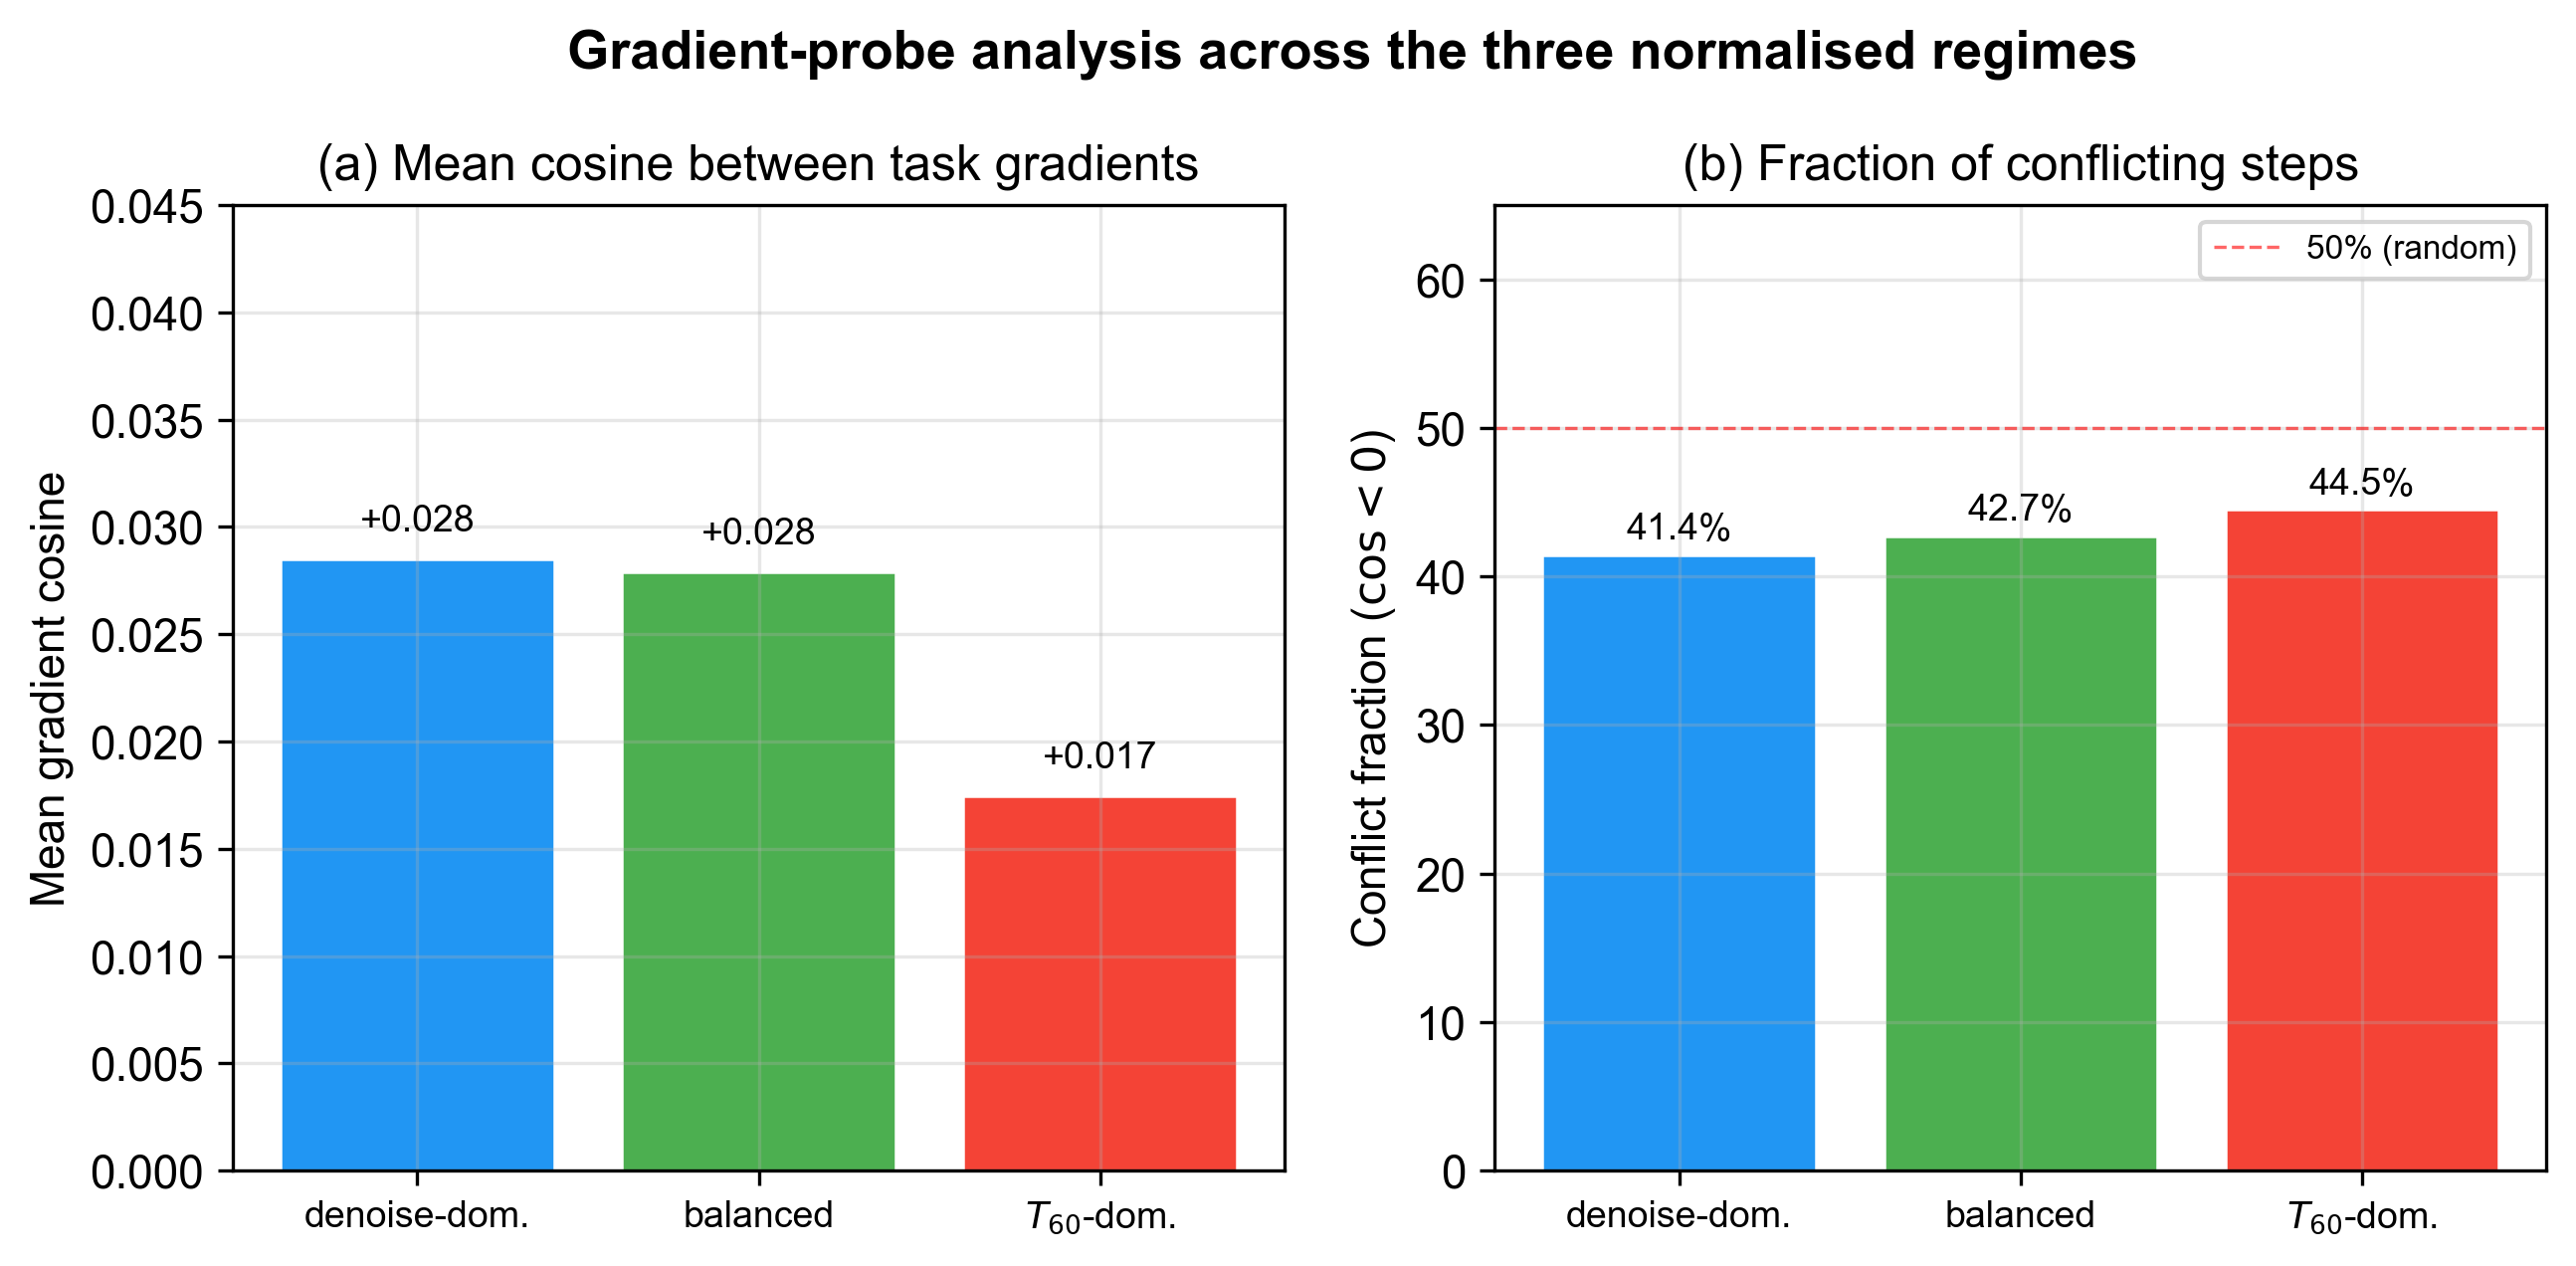
\includegraphics[width=0.95\textwidth]{figs/gradient_cos_r.png}
  \caption{Gradient cosine $\cos$ between the two task gradients on the
  shared encoder, across the three normalised regimes. (a) Mean $\cos$
  over training, all near $0$: the two tasks are neither cooperative nor
  systematically antagonistic. (b) Fraction of conflicting steps
  ($\cos<0$), well below $50\%$.}
  \label{fig:gradient}
\end{figure}

To check that the two tasks do not interfere antagonistically, we use
the gradient probe of Section~\ref{sec:exp:impl} to measure the cosine
$\cos$ between the two task gradients on the shared encoder throughout
training. As Fig.~\ref{fig:gradient} shows, $\cos$ stays centred near
$0$ (mean $\lvert\cos\rvert\approx 0.10$, with only $\sim$$41$\,\% of
steps having $\cos<0$): the two task gradients are nearly orthogonal,
neither cooperatively aligned nor in systematic conflict. The two tasks
can therefore be optimised jointly without one interfering with the
other, and what governs $T_{60}$ accuracy is the task-weight
ratio---i.e.\ how much the denoising task is allowed to shape the shared
representation---rather than any gradient conflict. How this shaping
actually takes place at the representation level is examined in
Section~\ref{sec:res:repr}.

\subsection{Representation analysis}\label{sec:res:repr}

To examine how the denoising auxiliary supervision reshapes the shared
representation, we apply CKA (feature similarity between each
multi-task configuration and the single-task baseline, per layer) and
linear probing (freeze the model, read out $T_{60}$ by ridge regression
on frozen layer features, and report the linearly decodable $T_{60}$
information as $R^{2}$). CKA is computed deterministically over the
full feature Gram matrix; the probe is averaged over five random 80/20
splits (mean $\pm$ SD) and is additionally evaluated in a deterministic
leave-one-split-out protocol, and the two protocols agree.

\begin{figure}[H]
  \centering
  \includegraphics[width=0.72\textwidth]{figs/cka_comparison.png}
  \caption{Linear CKA between each multi-task configuration and the
  single-task baseline, per shared layer (macro average over
  test1--test4; error bars denote the SD across the four test sets).
  Lower CKA indicates the denoising supervision has driven the
  representation further away from the single-task solution.}
  \label{fig:cka}
\end{figure}

\begin{figure}[H]
  \centering
  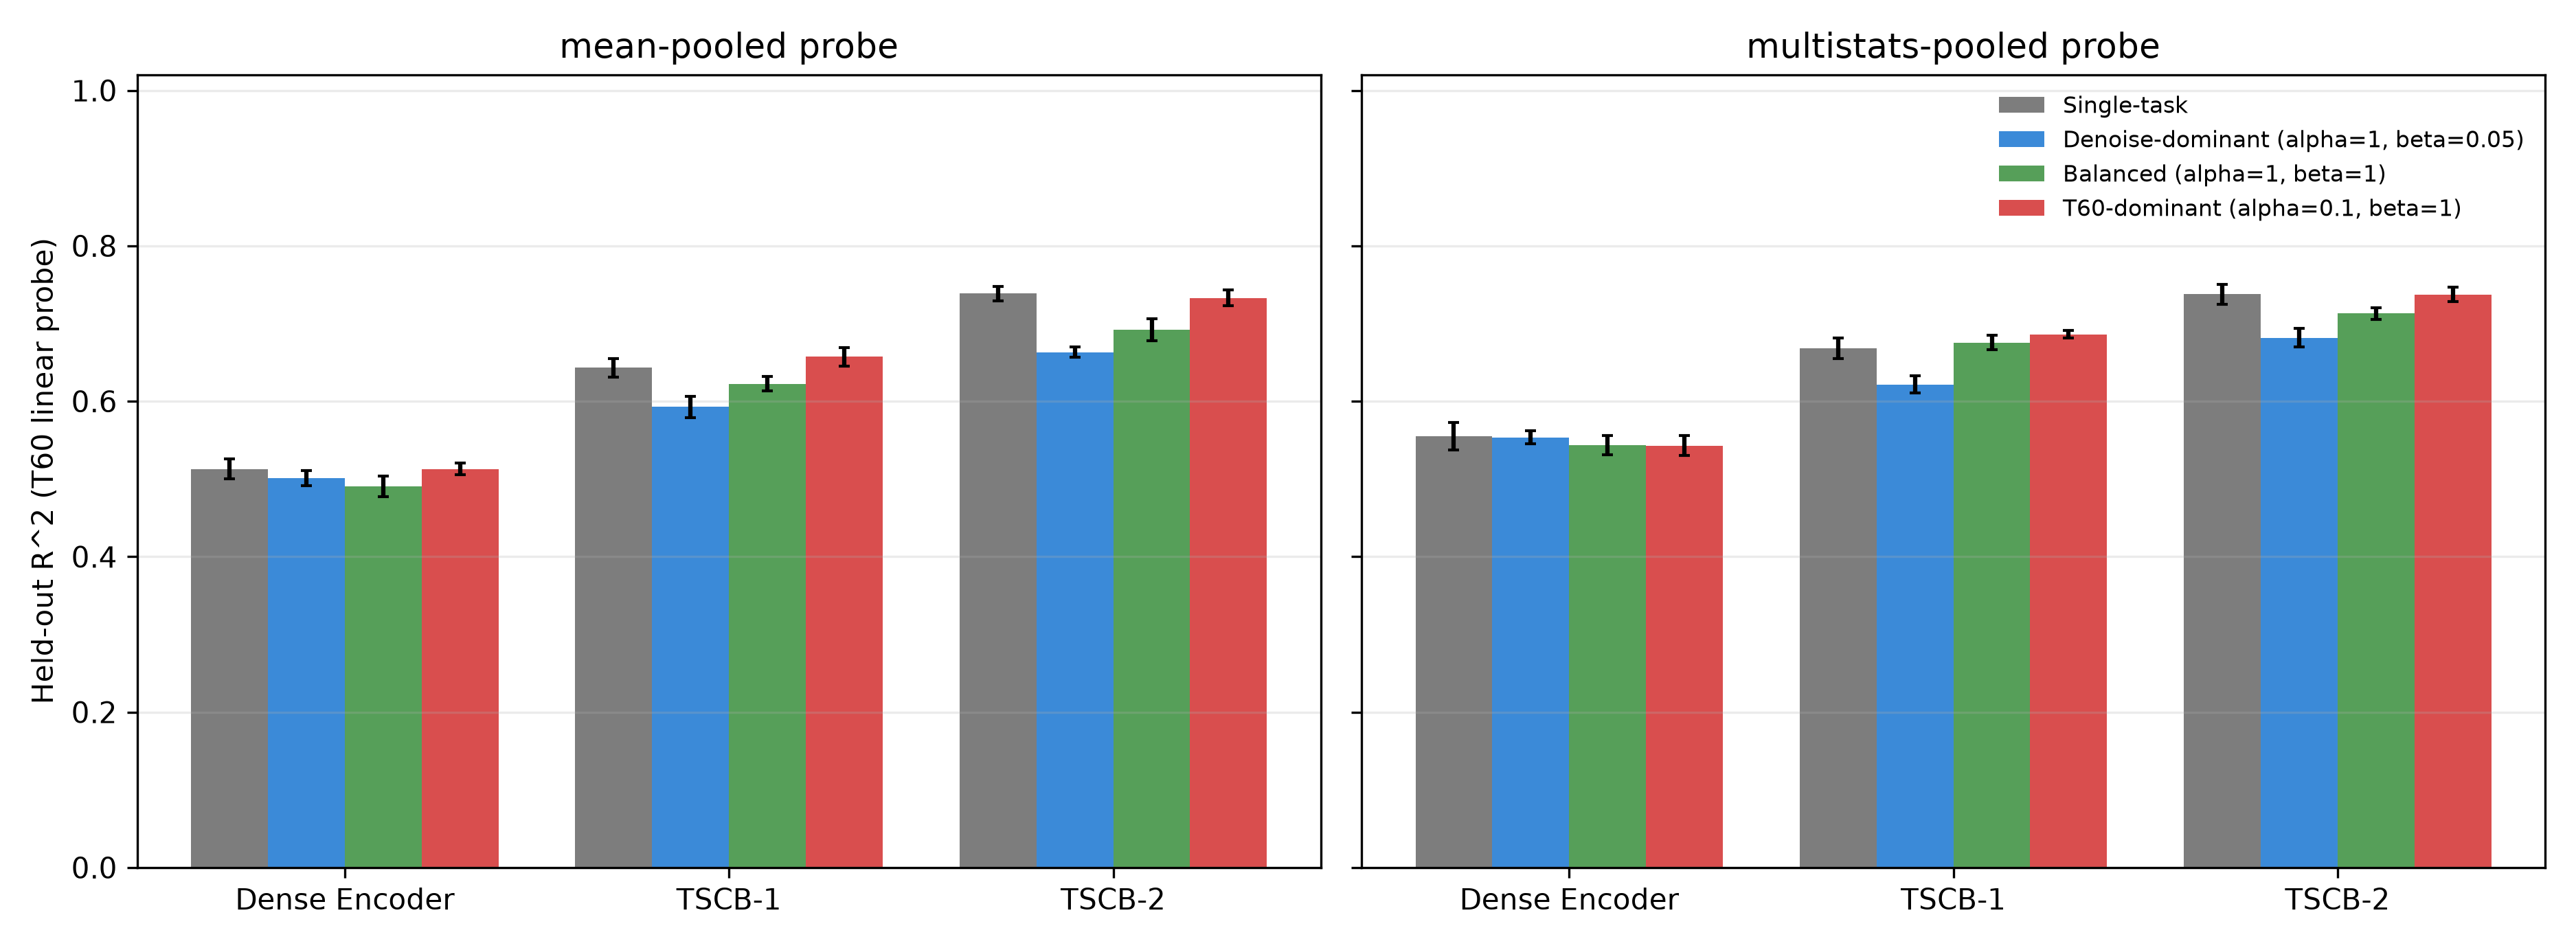
\includegraphics[width=0.95\textwidth]{figs/linear_probe.png}
  \caption{Linear probing $R^{2}$ per shared layer (Encoder / TSCB$_1$ /
  TSCB$_2$): single-task baseline vs.\ the three multi-task regimes
  (pooled 80/20 protocol, mean $\pm$ SD over five seeds). Left: global
  mean pooling; right: multi-statistic pooling (avg/max/std over time),
  which mirrors how the $T_{60}$ head reads the bottleneck.}
  \label{fig:linearprobe}
\end{figure}

CKA reveals a clear, depth-graded pattern that is consistent across all
four test sets. The encoder representation remains highly similar to
the single-task baseline for every regime (macro-averaged CKA $\geq
0.95$), whereas the divergence grows markedly deeper in the network.
At TSCB$_2$, the denoise-dominant regime ($\alpha{=}1.0,\beta{=}0.05$)
departs furthest from the single-task solution (macro CKA $0.51$;
$0.47$--$0.55$ across the four test sets, with paired-bootstrap $95\%$
confidence intervals supporting the same layer-wise trend), the balanced
regime is intermediate ($0.70$), and the $T_{60}$-dominant regime
($\alpha{=}0.1,\beta{=}1.0$), in which the denoising gradient is
suppressed, stays closest ($0.81$). This ordering of CKA coincides with
the ordering of $T_{60}$ accuracy in Table~\ref{tab:weight}
(denoise-dominant best, $T_{60}$-dominant worst): the more the
denoising gradient reshapes the shared representation, the lower the
$T_{60}$ RMSE. In other words, \emph{a stronger denoising gradient does
more than add a second objective; it actively reshapes the shared
representation, and this reshaping is what the $T_{60}$ head benefits
from.}

Linear probing (Fig.~\ref{fig:linearprobe}) adds the complementary
question of whether the reshaped representation is easier for a simple
linear reader to exploit. A ridge probe is fitted on frozen layer
features under two pooling schemes, of which the multi-statistic one
mirrors how the $T_{60}$ head reads the bottleneck. Three observations
follow. First, $T_{60}$ decodability accumulates with depth for every
model (Encoder $<$ TSCB$_1$ $<$ TSCB$_2$). Second, the denoise-dominant
model does not increase linear decodability: at TSCB$_2$ its $R^{2}$ is
$0.68\pm0.01$, slightly below the single-task baseline
($0.74\pm0.01$), with the balanced and $T_{60}$-dominant regimes in
between and an ordering that matches the supervision structure.
Third, this stands in contrast to the end-to-end results, in which the
same model attains the best RMSE. Read together with the
regression-head ablation of Section~\ref{sec:res:ablation}, where the
Fourier-KAN head clearly outperforms an MLP head under the identical
multi-task setting, this indicates that the multi-task gain does not
arise from adding linearly separable $T_{60}$ information; it arises
from a reshaped representation whose benefit is realised through the
non-linear Fourier-KAN readout.

\subsection{Results comparison with baselines}\label{sec:res:main}

We compare the proposed model (normalised main model, denoise-dominant
$\alpha=1.0,\beta=0.05$, determined by the weight tuning of
Section~\ref{sec:res:ablation}) with three blind $T_{60}$ estimators
(BERP, noiseaware, DAMTL) and the single-task ablation baseline on the
four test sets; the averaged metrics are reported in
Table~\ref{tab:main}.

\begin{table}[!htbp]
  \centering
  \caption{Main comparison on T60\_Dataset\_v7 (average over
  test1--test4; RMSE/MAE in ms).}
  \label{tab:main}
  \begin{tabular}{lcccc}
    \toprule
    Method & RMSE $\downarrow$ & MAE $\downarrow$ & $r$ $\uparrow$ & $R^{2}$ $\uparrow$ \\
    \midrule
    BERP~\citep{wang2025berp}              & 147.20 & 90.70 & 0.9035 & 0.8001 \\
    noiseaware~\citep{zheng2022noiseaware} & 133.66 & 82.38 & 0.9196 & 0.8451 \\
    DAMTL~\citep{zhang2024damtl}           & 138.94 & 86.07 & 0.9134 & 0.8323 \\
    Single-task KAN (ablation)             & 111.15 & 72.40 & 0.9484 & 0.8931 \\
    \textbf{Proposed (normalised)}         & \textbf{92.91} & \textbf{56.68} & \textbf{0.9625} & \textbf{0.9253} \\
    \bottomrule
  \end{tabular}
\end{table}

The proposed model outperforms the three comparison methods and the
single-task baseline on all four test sets (test1--4 = simulated/real
RIR $\times$ seen/unseen noise), confirming the effectiveness and
cross-condition robustness of the denoising auxiliary task with
normalised multi-task training.

\subsection{Effect of SNR on estimation accuracy}\label{sec:res:snr}

Table~\ref{tab:snr} reports the per-SNR-bin RMSE of the proposed model
and the three baselines, broken down by test-set scenario (simulated vs.\
real RIR).

\begin{table}[!htbp]
  \centering
  \caption{RMSE (ms) per SNR bin. Each scenario groups the two test sets
  sharing that RIR type; ``Avg.'' averages over all four test sets.
  Best per cell in \textbf{bold}.}
  \label{tab:snr}
  \setlength{\tabcolsep}{4pt}
  \begin{tabular}{llcccccc}
    \toprule
    Scenario & Method & $-5$\,dB & $0$\,dB & $5$\,dB & $10$\,dB & $\geq 15$\,dB & Avg. \\
    \midrule
    \multirow{4}{*}{\shortstack[l]{Sim.~RIR\\(test1+3)}}
      & BERP       & 225.5 & 150.7 & 108.8 & 111.7 & 111.2 & 143.0 \\
      & DAMTL      & 203.1 & 158.1 & 115.2 & 102.0 & 110.7 & 138.1 \\
      & noiseaware & 204.8 & 166.7 & 100.1 & 87.8  & 79.5  & 129.1 \\
      & Proposed   & \textbf{132.2} & \textbf{93.2} & \textbf{65.5} & \textbf{70.1} & \textbf{81.8} & \textbf{90.1} \\
    \midrule
    \multirow{4}{*}{\shortstack[l]{Real RIR\\(test2+4)}}
      & BERP       & 242.2 & 180.0 & 139.3 & 98.9  & 94.3  & 151.7 \\
      & DAMTL      & 232.6 & 169.4 & 121.9 & 85.3  & 82.3  & 140.5 \\
      & noiseaware & 238.5 & 159.2 & 115.1 & 78.9  & 81.1  & 138.4 \\
      & Proposed   & \textbf{144.7} & \textbf{111.0} & \textbf{82.1} & \textbf{68.5} & \textbf{71.6} & \textbf{95.7} \\
    \midrule
    \multirow{4}{*}{\shortstack[l]{All\\(test1--4)}}
      & BERP       & 234.0 & 166.0 & 125.0 & 105.5 & 103.1 & 147.4 \\
      & DAMTL      & 218.3 & 163.9 & 118.6 & 94.0  & 97.5  & 139.3 \\
      & noiseaware & 222.3 & 163.0 & 107.9 & 83.5  & 80.3  & 133.8 \\
      & \textbf{Proposed} & \textbf{138.6} & \textbf{102.5} & \textbf{74.3} & \textbf{69.3} & \textbf{76.9} & \textbf{93.0} \\
    \bottomrule
  \end{tabular}
\end{table}

\subsection{Effect of reverberation time on estimation accuracy}\label{sec:res:t60bin}

Table~\ref{tab:t60bin} reports the per-$T_{60}$-bin RMSE of the proposed
model and the three baselines, broken down by test-set scenario.

\begin{table}[!htbp]
  \centering
  \caption{RMSE (ms) per $T_{60}$ bin (s). Each scenario groups the two
  test sets sharing that RIR type; ``Avg.'' averages over all four test
  sets. Best per cell in \textbf{bold}.}
  \label{tab:t60bin}
  \setlength{\tabcolsep}{5pt}
  \begin{tabular}{llccccc}
    \toprule
    Scenario & Method & $0.1$--$0.4$ & $0.4$--$0.7$ & $0.7$--$1.0$ & $1.0$--$1.5$ & Avg. \\
    \midrule
    \multirow{4}{*}{\shortstack[l]{Sim.~RIR\\(test1+3)}}
      & BERP       & 88.5  & 117.9 & 163.0 & 261.1 & 143.0 \\
      & DAMTL      & 97.1  & 110.4 & 136.6 & 278.4 & 138.1 \\
      & noiseaware & 94.0  & 107.1 & 155.3 & 205.3 & 129.1 \\
      & Proposed   & \textbf{64.1} & \textbf{80.6} & \textbf{96.0} & \textbf{155.0} & \textbf{90.1} \\
    \midrule
    \multirow{4}{*}{\shortstack[l]{Real RIR\\(test2+4)}}
      & BERP       & 88.1  & 140.0 & 176.0 & 331.9 & 151.7 \\
      & DAMTL      & 95.9  & 98.1  & 160.5 & 313.2 & 140.5 \\
      & noiseaware & 92.9  & 111.7 & 156.4 & 301.0 & 138.4 \\
      & Proposed   & \textbf{65.7} & \textbf{83.3} & \textbf{105.1} & \textbf{203.3} & \textbf{95.7} \\
    \midrule
    \multirow{4}{*}{\shortstack[l]{All\\(test1--4)}}
      & BERP       & 88.3  & 130.9 & 168.8 & 294.8 & 147.4 \\
      & DAMTL      & 96.5  & 103.6 & 147.5 & 294.3 & 139.3 \\
      & noiseaware & 93.4  & 109.7 & 155.8 & 252.6 & 133.8 \\
      & \textbf{Proposed} & \textbf{65.0} & \textbf{82.2} & \textbf{100.1} & \textbf{178.2} & \textbf{93.0} \\
    \bottomrule
  \end{tabular}
\end{table}

\subsection{Denoising results}\label{sec:res:denoise}

Table~\ref{tab:denoise} reports the denoising quality of the three
normalised regimes, averaged over test1--test4. Per the target defined
in Section~\ref{sec:method:denoise}, these metrics reflect noise removal
while preserving the reverberation.

\begin{table}[!htbp]
  \centering
  \caption{Denoising metrics for the three normalised regimes (average
  over test1--test4).}
  \label{tab:denoise}
  \begin{tabular}{lcccc}
    \toprule
    Regime & PESQ $\uparrow$ & STOI $\uparrow$ & SI-SDR (dB) $\uparrow$ & $\Delta$SI-SDR \\
    \midrule
    Noisy input                & 2.721 & 0.847 & 15.91 & --- \\
    \midrule
    $T_{60}$-dominant          & 3.077 & 0.891 & 18.80 & +2.89 \\
    Balanced                   & 3.178 & 0.907 & 19.79 & +3.88 \\
    \textbf{Denoise-dominant (proposed)} & \textbf{3.472} & \textbf{0.928} & \textbf{21.13} & \textbf{+5.21} \\
    \bottomrule
  \end{tabular}
\end{table}

The proposed denoise-dominant model removes additive noise while
preserving the reverberation, yielding gains of $+0.75$ PESQ, $+0.08$
STOI and $+5.21$\,dB SI-SDR over the noisy input. Crucially, the
denoising quality follows the \emph{same} ordering as the $T_{60}$
accuracy (Table~\ref{tab:weight}): the denoise-dominant regime is best
at both tasks, and the $T_{60}$-dominant regime is worst at both. There
is therefore no trade-off between the auxiliary and the main
task---giving the denoising task a larger weight improves the two tasks
jointly, consistent with the task-weight ablation of
Section~\ref{sec:res:weight}.

% =====================================================================
\section{Conclusion}\label{sec:conclusion}
% =====================================================================

We proposed a multi-task learning framework for blind $T_{60}$
estimation that pairs $T_{60}$ regression (main task) with denoising
reconstruction (auxiliary task) over a shared dual-path time--frequency
Conformer backbone, with a Fourier-KAN head for $T_{60}$ estimation.
The main findings are: (1) the denoising auxiliary task, at the cost of
about $0.54$\,M decoder parameters, reduces the $T_{60}$ RMSE
substantially relative to the single-task ablation baseline
($111.15$\,ms) and outperforms BERP, DAMTL and noiseaware; (2) gradient
probing shows that the two task gradients are nearly orthogonal with no
systematic conflict, so the two tasks can be optimised jointly without
interference, and a task-weight ablation together with representation
analysis shows that the gain stems from the denoising task reshaping the
shared representation: among the tested weight configurations, those
departing further from the single-task solution attain lower RMSE; (3)
the Fourier-KAN head outperforms an MLP head under comparable settings.
Representation analysis (CKA and linear probing) further reveals this
reshaping mechanism: the denoise-dominant regime departs furthest from
the single-task solution (lowest CKA), yet the $T_{60}$ cue remains
highly linearly decodable, though not more so than in the single-task
baseline. Together with the head ablation, this indicates that
denoising re-encodes rather than removes the $T_{60}$ information, and
that the benefit of the reshaped representation is realised through the
non-linear Fourier-KAN readout.

Future work may explore finer-grained weight sweeps and adaptive
gradient balancing (e.g., GradNorm), replacing or extending denoising
with other auxiliary tasks (e.g., dereverberation, sound-event
detection), and deployment evaluation on real-world recordings.

\bibliographystyle{cas-model2-names}
\bibliography{refs}

\end{document}
